\documentclass[12pt]{article}
\usepackage{amsmath}
\usepackage{amssymb}
\usepackage{amsbsy}
\usepackage{bm}
\usepackage{amsthm}
\usepackage{comment}
\usepackage{hhline}
\usepackage[left=1.5cm, right=1.5cm, bottom=1.5cm, top=1.5cm]{geometry}
\usepackage{graphicx}
\usepackage{algpseudocodex}
\newcommand{\tarc}{\mbox{\large$\frown$}}
\newcommand{\arc}[1]{\stackrel{\tarc}{#1}}
\usepackage{arcs}
\usepackage{pgf}
\usepackage{tikz}
\usepackage{pgfpages}
\newcommand{\nobarfrac}{\genfrac{}{}{0pt}{}}
\pgfpagesdeclarelayout{boxed}
{
  \edef\pgfpageoptionborder{0pt}
}
{
  \pgfpagesphysicalpageoptions
  {%
    logical pages=1,%
  }
  \pgfpageslogicalpageoptions{1}
  {
    border code=\pgfsetlinewidth{2pt}\pgfstroke,%
    border shrink=\pgfpageoptionborder,%
    resized width=.95\pgfphysicalwidth,%
    resized height=.95\pgfphysicalheight,%
    center=\pgfpoint{.5\pgfphysicalwidth}{.5\pgfphysicalheight}%
  }%
}
\usepackage{hyperref}
\hypersetup{
    colorlinks=true,
    linkcolor=blue,
    filecolor=magenta,      
    urlcolor=cyan,
    pdftitle={Overleaf Example},
    pdfpagemode=FullScreen,
    }

\pgfpagesuselayout{boxed}
\date{}
\title{\textbf{Racial Bias}}
\author{Armaan Khetarpaul}
\begin{document}
\maketitle
\hrule height 2pt \relax
\section{Fake it till you make it: face analysis in the wild using synthetic data alone}
We describe how to synthesize realistic and diverse training data for face analysis in the wild, achieving results in line with the state of
the art. Second, we present ablation studies that validate the
steps taken to achieve photorealism. Third is the synthetic dataset itself.\\
Common approach to generate synthetic data is 3D Morphable Model
(3DMM), since these can provide consistent labels for
different faces. These approaches only render part of the face, the resulting
data has limited use for tasks that consider the whole face.\\
An alternative is to render 3D scans directly. BU-4DFE dataset and commercially-available 3D head scans for head pose estimation are very realistic, these approaches are limited by
the diversity expressed in the scans themselves, and cannot
provide rich semantic labels for machine learning.\\
Manipulating 2D images can be an alternative to using
a 3D graphics pipeline. These approaches can only make
minor adjustments to existing images, limiting their use.\\
\\
Synthetic data is rarely used on its
own for face-related machine learning, because of domain gap. Learned domain adaptation modifies synthetic images
to better match the appearance of real images. Instead of adapting data, it is possible to learn features
that are resistant to the differences between domains.\\
\subsection{Synthesizing Face Images}
We use procedural
generation to randomly create and render novel 3D faces
without any manual intervention. We start by sampling a generative 3D face model that
captures the diversity of the human population. We then randomly `dress up' each face with samples from large collections of hair, clothing, and accessory assets. 
\subsubsection{3D Face Model}
Base model has 7667 vertices, 7414 polygons and 4 joints.\\
The Mesh Generating Function $\mathcal{M}$ takes $\vec{\beta}$ for identity, $\vec{\psi}$ for expression, $\vec{\theta}\in \mathbb{R}^{3\times \text{ no. of joints}}$ for pose and outputs a 3D mesh in $\mathbb{R}^{3\times\text{ no.of mesh vertices}}$.
\[\mathcal{M}(\vec{\beta},\vec{\psi},\vec{\theta})=\mathcal{L}(\mathcal{T}(\vec{\beta},\vec{\psi}),\vec{\theta},\mathcal{J}(\vec{\beta});W)\]
where $\mathcal{L}(X,\vec{\theta}, J;W)$ is a standard linear blend skinning
(LBS) function that rotates vertex positions $X$ about joint locations $J$ by local joint rotations $\vec{\theta}$,
with per-vertex weights $W$ determining how rotations are interpolated across the mesh. $\mathcal{T}$ constructs a face mesh in the bind pose by adding
displacements to the template mesh $T$ given linear identity basis $S$ and expression
basis $E$. $\mathcal{J}$ moves the template joint locations $J$ to account for changes in identity.
\subsubsection{Expression}
We apply random expressions to each face so that our
downstream machine learning models are robust to facial motion. Expressions are obtained from a library of 27000 parameters and sample expressions from a manually animated sequence that was designed to fill the gaps in
our expression library by exercising the face in realistic.
\subsubsection{Texture}
From cleaned face scans, textures are collected. We extract one
albedo texture for skin color, and two displacement maps. The coarse displacement map encodes scan
geometry that is not captured by the sparse nature of our
vertex-level identity model. The meso-displacement map
approximates skin-pore level detail and is built by high-pass
filtering the albedo texture, assuming that dark pixels correspond to slightly recessed parts of the skin.
\subsubsection{Hair}
Represent hair as
individual 3D strands, with a full head of hair comprising
over 100,000 strands. Modelling hair at the strand level
allows us to capture realistic multi-path illumination effects. r hair library includes 512 scalp hair
styles, 162 eyebrows, 142 beards, and 42 sets of eyelashes.
Each asset was authored by a groom artist who specializes in
creating digital hair. At render time, we randomly combine
scalp, eyebrow, beard, and eyelash grooms.
\subsubsection{Clothing}
Digital wardrobe
contains 30 upper-body outfits which were manually created
using clothing design and simulation software. In addition to upper-body garments, we
dress our faces in headwear (36 items), facewear (7 items)
and eyewear (11 items) including helmets, head scarves, face
masks, and eyeglasses.
\subsubsection{Rendering}
We render face images with Cycles, a photorealistic raytracing renderer. We randomly position a camera around
the head, and point it towards the face and  employ image-based lighting with high dynamic range images (HDRI) to illuminate the face and
provide a background.
\subsection{Analysis}
We evaluate our synthetic data on two common face analysis tasks: face parsing and landmark localization.
\subsubsection{Method}
We render a single training dataset for both landmark
localization and face parsing, comprising 100,000 images at
512×512 resolution. During training, we perform data augmentation including
rotations, perspective warps, blurs, modulations to brightness
and contrast, addition of noise, and conversion to grayscale.
\subsubsection{Parsing}
Face parsing assigns a class label to each pixel in an
image, e.g. skin, eyes, mouth, or nose. Benchmark using Helen and LaPa datasets.\\
Method We treat face parsing as image-to-image translation. Given an input color image $x$ containing C classes,
we wish to predict a C-channel label image $\hat{y}$ of the same
spatial dimensions that matches the ground truth label image $y$. Pixels in $y$ are one-hot encoded with the index of the
true class. For this, we use a UNet with ResNet-18
encoder. We train this network with synthetic data
only, minimizing a binary cross-entropy (BCE) loss between
predicted and ground truth label images.\\
We use label adaptation. Label adaptation transforms labels
predicted by our face parsing network (trained with synthetic
data alone) into labels that are closer to the distribution in
the real dataset. We treat label adaptation
as another image-to-image translation task, and use a UNet
with ResNet18 encoder.\\
It can be seen that training
with synthetic data alone produces comparable results to
training with real data.
\begin{center}
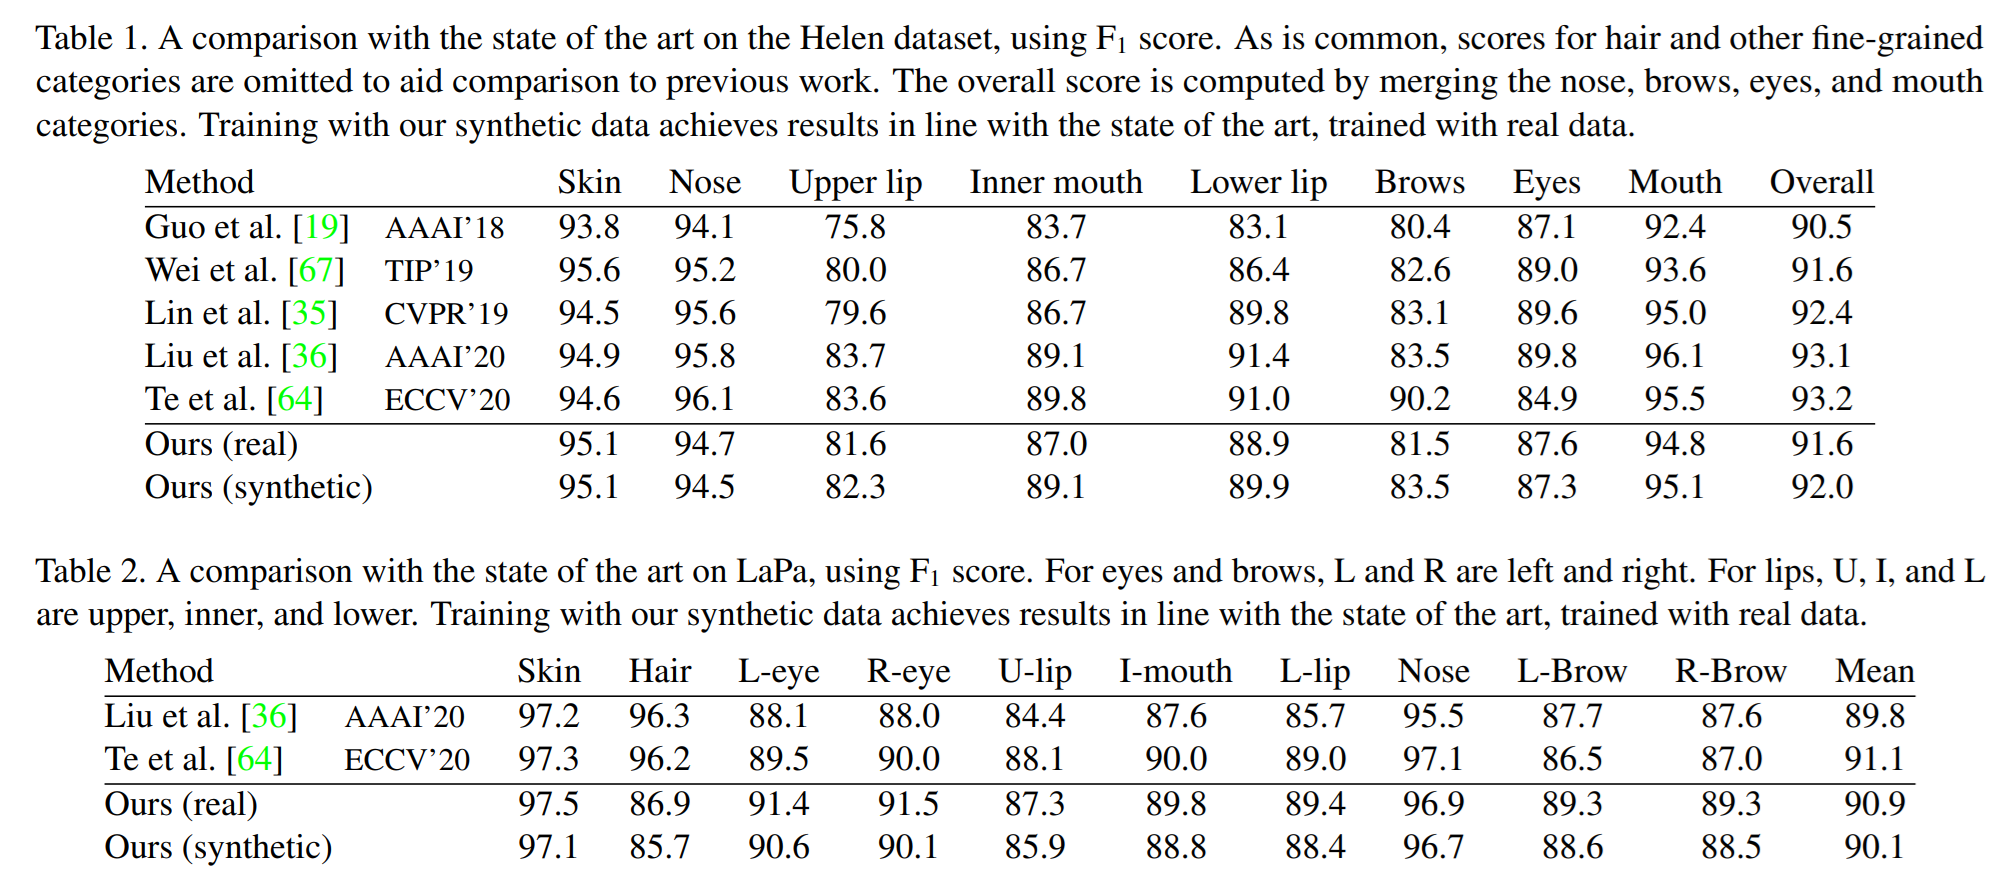
\includegraphics[scale = 0.7]{img1.png}
\end{center}
Landmark localization finds the position of facial points
of interest in 2D. We evaluate our approach on the
300W dataset, which is split into common (554 images), challenging (135 images) and private (600 images)
subsets.\\
Method We train a ResNet34 with mean squared
error loss to directly predict 68 2D landmark coordinates
per-image. Label adaptation is performed using a two-layer perceptron to address systematic differences between synthetic
and real landmark labels.\\
The network trained with our synthetic data can detect landmarks with accuracy comparable to recent methods trained with real data.
Comparison to real data We apply our training methodology (including data augmentations and label adaptation) to
the the training and validation portions of the 300W dataset,
to more directly compare real and synthetic data.
\begin{center}
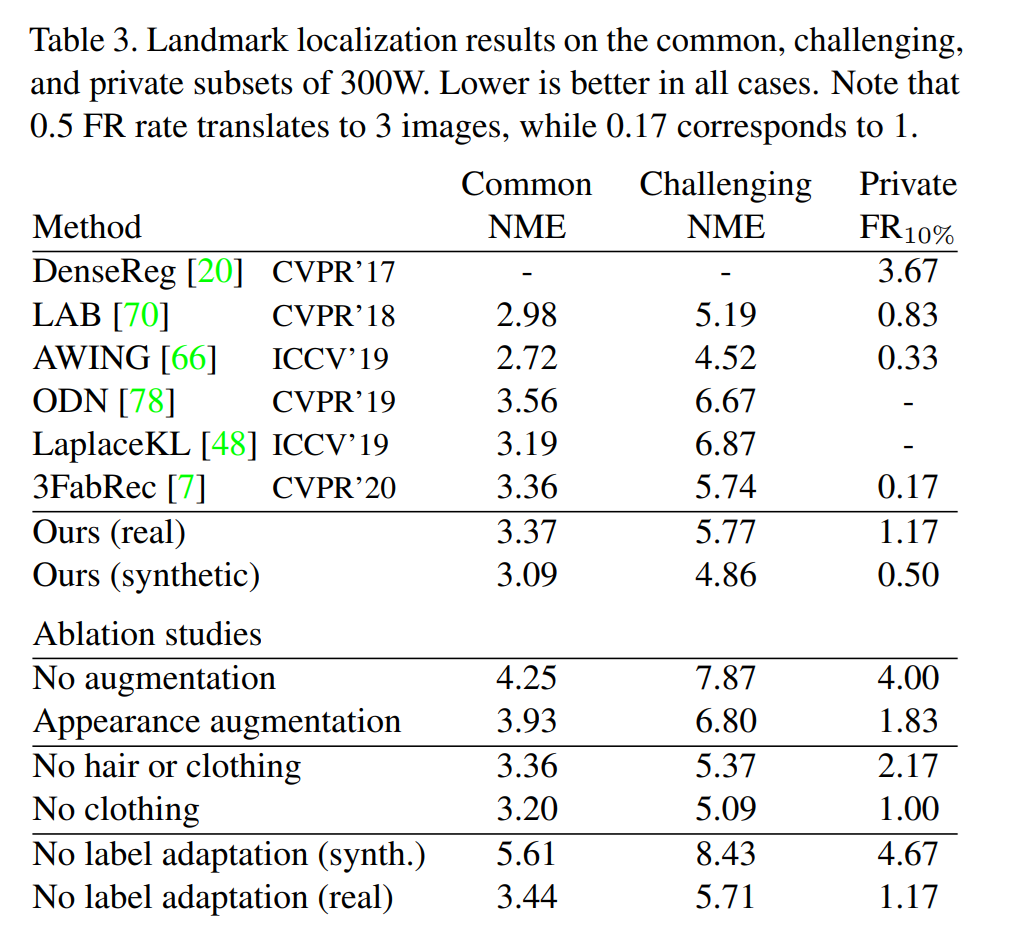
\includegraphics[scale = 0.7]{img2.png}
\end{center}
\subsection{Discussion}
Landmark localization improves as we increase the number of training images. We study the importance of data augmentation when
training models on synthetic data. We train models with:
1 no augmentation; 2 appearance augmentation only (e.g.
colour shifts, brightness and contrast); 3 full augmentation,
varying both appearance and geometry (e.g. rotation and
warping). When evaluating models trained on synthetic data - using
label adaptation to improve label consistency reduces error. If we remove clothing and hair, landmark accuracy suffers.
\section{Analyzing and Reducing the Damage of Dataset Bias
to Face Recognition with Synthetic Data}
Problems:
\begin{enumerate}
  \item Difficult to
  systematically analyze the effects of dataset bias on the generalization performance.
  \item Deep face recognition systems do not generalize well across benchmarks, due to the severe sampling
  biases in public datasets. This
  causes well-known problems such as a lack of diversity and
  fairness in face recognition 
\end{enumerate}
We explore two complementary application areas
for synthetic face images:
\begin{enumerate}
  \item Using fully annotated synthetic face images we can study the face recognition rate as a function of interpretable parameters such as face pose.
  \item We pre-train neural networks with large-scale synthetic data that is highly variable in face pose and the number of facial identities.
\end{enumerate}
\subsection{Face Image Generator}
We use the Basel Face Model 2017 (BFM2017) which is learned from 200 neutral face scans and
160 expression deformations. Natural looking, three dimensional faces with expressions can be generated by sampling
from the statistical distribution of the model. The proposed generator
enables us to generate infinite amount of face images with
detailed labeling of the most relevant sources of image variation.
\subsection{Analysis}
We get the total
recognition rate (TRR) as a function along the axis of nuisance transformations.
\subsubsection{Setup}
We simulate strong background variations,
which are common in real world data, by sampling random
textures from our empirical background model. All other
nuisance parameters are fixed. After splitting, we bias the train set, train DCNNs on it and evaluate
how well the DCNNs generalize to the unbiased test data. We test these networks at the task of face classification. Thus, the task is to recognize a face from an image,
for which the identity is known at training time. We focus on diagnosing the performance of
DCNNs on the task that they were explicitly optimized on.\\
\\
The size of the images is set to
$227 \times 227$ pixels. We train the DCNNs with stochastic gradient descent (SGD) and backpropagation with the Caffe
deep learning framework via the Nvidia DIGITS training system. Every DCNN is trained from scratch for 30
epochs with a base learning rate of $l = 0$.001 which is multiplied every 10 epochs by $\gamma = 0.1$. For the yaw pose, we sample the parameter space at intervals of $\tfrac{\pi}
{32}$ radian and for the direction
of light at $\tfrac{\pi}
{16}$ radian. Each face image is overlayed on 50
different background textures in the training as well as in
the test set.
\subsubsection{EXP-1: Bias in the range of the yaw pose}
We limit the range of the yaw pose in
the training data to $\left[-45,45\right]$ and $\left[-90,0\right]$. The light direction is fixed to be frontal. Both DCNNs achieve high recognition rates for the observed yaw
poses. However, the recognition performance drops significantly when faces are outside of the observed pose range. The VGG-16
network achieves higher overall recognition rates, because
it generalizes better to larger unseen yaw poses.
\subsubsection{EXP-2: Sparse sampling of the yaw pose.}
We first bias
the training set to yaw poses of -45
and 45. VGG-16 achieves a TRR of 70.5\% at test time, whereas AlexNet
only achieves 51.8\%. VGG-16 achieves
constantly higher recognition rates across all poses. If we add frontal faces at training time VGG-16 achieves a TRR of 81.9\%,
whereas AlexNet achieves 69.3\%. Remarkably, VGG16 is now able to recognize all faces correctly across the
full range of [-45
, 45], whereas the recognition rates
of AlexNet still drop significantly for poses in between
[-45, 0] and [0
, 45].
\subsubsection{EXP-3: Disentanglement of pose variation}
Here half of the identities in the training set vary in the
yaw pose range of [-90, 0] (left) and the other half in the range of [0, 90] (right). We evaluate the Left-identities and
Right-identities separately. We observe, that the DCNNs only slightly improve compared to
setup where the yaw pose range is restricted to [-90, 0]
for all identities (dotted curves). Thus, both DCNNs cannot
benefit from the additional information in the training set.
\subsubsection{Analysis with Synthetic Data}
Deeper networks generalize better to unseen head poses. A major reason why VGG-16 outperforms AlexNet
at face recognition is that it can generalize better to faces in
previously unseen face poses\\
\\
Deep networks cannot disentangle face pose from facial identity. A major limitation of the analyzed DCNN architectures is that they have severe difficulties to generalize
when facial identities do not share the same pose variation. Thus, deep networks cannot disentangle well
the image variation caused by changes in the face pose from
the one induced by changes in the facial identity.
\subsection{Reducing Damage from Bias}
\subsubsection{Setup}
OpenFace framework. For face detection
and alignment we use a publicly available multi-task CNN 2. We train the FaceNetNN4 architecture with the vanilla setting, as provided in the OpenFace
framework. The aligned images are scaled to $96\times96$ pixels. The triplet loss is trained with batches of 20 identities and
15 sample images per identity for 200 epochs. The real-world training data for face recognition is sampled from the cleaned Casia WebFace dataset.\\
\\
Synthetic face image generation. The head pose is sampled according to a uniform
pose distribution on the yaw, pitch and roll angles in the respective ranges $r_{yaw} =$ [-90, 90], $r_{pitch}$ = [-30, 30]
and $r_{roll} = $[-15, 15]. For face recognition, we generate
one million face images with 20K different identities and
100 example images per identity.
\subsubsection{Biases}
For real data, we observe that the distribution of the training data
is similar to some benchmark datasets. For synthetic data, we observe
that for the CMU-Multi-PIE benchmark the performance is
similar to that of a deep network trained with real-world data . This suggests that our synthetic face images can well
represent the facial appearance in constrained visual environments.\\
\\
In real data some facial properties such as head pose, illumination or facial expression
are difficult to annotate and therefore cannot be taken into
account when collecting data. In synthetic data, these properties can be modeled very well and thus can be sampled
extensively, however, other characteristics of faces are currently not modeled with parametric face models.
\subsubsection{Priming}
We fine-tune the SYN-only model with different subsets (10\%, 25\%, 100\%) of the real-world training data. The
primed models considerably outperform the unprimed models at face recognition. Interestingly, even when fine-tuning
with the full real-world datasets the models still have an enhanced performance compared to the unprimed models. The real-to-virtual gap can almost be closed with 25%
of the real data. Remarkably, priming with synthetic data
leads to a performance increase across all benchmarks, even
though the individual datasets have very different imaging
characteristics.
\subsubsection{Discussion}
Enhanced generalization performance. Priming with
synthetic data followed by fine-tuning with real-world
data enhances the generalization performance consistently
across all benchmark datasets compared to training with
real-world data only.\\
\\
Enhanced data efficiency. Using our priming approach
the number of real-world data needed to achieve competitive performance at face recognition was reduced by 75\%.

\section{Synthetic Data for Face Recognition: Current State and Future
Prospects
}
Uses cases of synthetic data:
\begin{enumerate}
  \item Training FR: Modern FR solutions are based
  on deep learning models that are either trained
  directly to generate identity-discriminant feature
  representations or to classify the identity classes in the training data. If the model is trained in
  one of the two approaches mentioned above, then
  the synthetic data has to contain a large number
  of identities and multiple samples of each identity. If the model is trained on partially authentic data, however, the intra-class variation of this
  data is low, then the synthetic data needs to contain multiple samples for each of the authentic
  identities, i.e. act as an augmentation strategy.
  \item Evaluating FR: FR algorithmic evaluation requires the existence of a large set of genuine
  (same identity) and imposter (different identity)
  face image pairs that represent the real operational scenario. The need for a large number
  of these pairs is intensified by the ever-more
  accurate performance of FR algorithms. need for
  large-scale evaluation data is one of the main motivations behind requiring synthetic data for the
  evaluation.
  \item Attacking FR: Synthetic
  data can be created so that a certain face can
  be matched with two or more faces. This can
  target automatic FR comparison or human image verification, or both. Such attacks can be
  face morphing attacks, where an image is generated to match two or more identities, then used
  on an identity or travel document with the alphanumeric data of when the targeted matches.\\
  Another attack in the same category is the MasterFace attack, where the synthetic face is created to match a wider proportion
of the population, raising many security threats.\\
The second type of attack by generated face images might focus on generating a face image of a
specific identity. Such attacks are commonly referred to as Deep-Fakes and they are commonly
used to fool the viewer into wrongly believing
that a certain person has said or done an action
in an image or a video.\\
A third attack can use
synthetic faces that maintain a certain identity
but excludes a specific pattern with the aim of
attacking a biometric-based system that ensures
a legal operation of a process. 
  \item Enhancing the privacy for FR users: Although excluding certain patterns from generated images of specific identities can be seen as
  an attack on biometric systems, in different usecases, they can be seen as a privacy-enhancing
  tool when they are used to avoid the illegal or
  unconsented processing of the data. Such generation of the data aims at maintaining a certain
  set of visual patterns but removing the clues of a
  specific pattern.
\end{enumerate}

\subsection{What data is needed and
what properties make it
good?}
\begin{enumerate}
  \item Single faces of random identities: synthetic face images of random identities without the requirement of multiple images
  to belong to one identity can be used for training FR models in an unsupervised manner. They
  additionally can be used to evaluate FR models,
  specifically evaluate the FMR, especially when
  the targeted operational point is at a very low
  FMR, requiring an extremely large number of
  diverse imposter pairs to make the evaluation
  result statistically significant. Here, such data
  should be realistic, i.e. act like authentic data
  when processed by the FR model.
  \item Multiple faces per random identity: This
  kind of data represents what one would typically expect from FR training or evaluation data.
  That is, multiple identities, with multiple images per identity. Here, the data should possess an inter and intra-class variability of the targeted authentic data scenario.
  \item Multiple faces of an existing identity: Authentic face data with insufficient intra-class
  variation is problematic for the training and evaluation of FR. Such data will lead to models that are not trained
  to tolerate intra-class variation (e.g. pose, expressions, age, illumination, etc.) and thus are
  expected to lead to high FNMR in practical operations. Evaluation data
  in some practical cases such as an authority that
  possesses only a single (or few) images per identity would not be
  sufficient to evaluate the expected FNMR as no
  (or few) genuine pairs exist in the data. Both
  cases require acquiring more samples of each of
  the existing identities. These samples have to
  be of realistic variation that matches the targeted scenario.
  \item A face of multiple identities: A synthetic
  face can also be used as an attack, the fact that
  a face can be generated synthetically with properties that enables an attack on identity systems
  pursues researchers to foresee such attacks.\\
  A face can be synthesized in a way that it matches
  two more specific (known) identities to create
  what is referred to as a morphing attack.\\
  A wider attack that surfaced lately in the literature is the MasteFace attack, where the attack
image is synthesized to match a wide range of
the population without the need to know the
targeted identities  
\item A face of specific authentic identity: Synthesizing a face of a specific authentic identity
is usually related to the need to synthesize this
face with also a specific expression or domain,
unlike generating such faces of an authentic identity where a realistic variation is needed. This is
commonly related to what is referred to as DeepFake faces but also includes other face manipulation techniques such as expression and attribute
manipulations.
\item A face that excludes a specific pattern:
A face synthesizing process can maintain a subset of patterns from a specific face and excludes
other subsets of these patterns. Such patterns can be identity information, age, gender, ethnicity, or even the patterns that make a face detectable as a face, among other attribute patterns. Such a process can be seen as an attack
if it is aimed at avoiding a consented required
process, such as automatic age verification to receive a service or make an online purchase. However, such a process can also be seen as a privacy
enhancement mechanism. A subset of this is to exclude
the patterns of the face that makes it detectable
and thus avoid further processing.
\end{enumerate}
\subsection{SOTA}
\subsection{Face Image Generation}
Specifically, a deep generative model takes
random points from e.g. Gaussian distribution and
maps them through a neural network such as the
generated distribution closely matches the authentic
data distribution. GANs, VAEs, and DiffModels are the best ones.
\subsection{How do the DGM approaches
match the needed synthetic face
data properties?}
\begin{itemize}
  \item Single faces of random identities: DGM approaches such as StyleGAN presented very
  promising results in generating single faces of
  random synthetic identities with high visual fidelity. 
  \item Multiple faces per random identities: Approaches such as Face-ID-GAN, DiscoFaceGAN, GAN-Control, InterFaceGAN
, and CONFIG proposed GAN models based on disentangled representation learning
  to conditionally generate face images from synthetic identities with predefined attributes 
  \item Multiple faces of an existing identity: DGM approaches such as CONFIG are able to regenerate multiple faces of an existing identity
  by reconstructing input faces with a predefined
  set of attributes such as changing expression,
  wearing sunglasses, adding makeup, or changing
  hair color.
  \item Recent works such as MorGAN, MIPGAN,
  and MorDIFF, make use of generative models to generate a face of multiple identities by
  interpolating two or more latent vectors of synthetic or real faces and then generating a new
  face of multiple identities.
  \item • A face of specific authentic identity: DGM approaches that targeted image-to-image modeling achieved impressive results in generating a
  face of specific authentic identity. This has been
  commonly achieved by manipulating the input
  source face to match specific attributes or a target domain while maintaining the identity information of the source image.
  \item A face that excludes a specific pattern: None
  of the SOTA DGM approaches explicitly target
  generating a face that excludes a specific pattern.
  A number of works make use of DGM approaches
  to exclude a specific pattern e.g. identity, age, or
  gender of authentic input faces, especially when
  such models include attribute disentanglement.
\end{itemize}
\subsection{SOTA of Use-cases}
Very recently a few works build on existing DGM approaches to propose FR based on synthetic data. 
\begin{itemize}
  \item Training FR: Synthetically generated face data has been
  proposed as an alternative to privacy-sensitive authentic data to train FR models mitigating the technical, ethical, and legal concerns of using authentic biometric data in training FR models.
  \begin{center}
    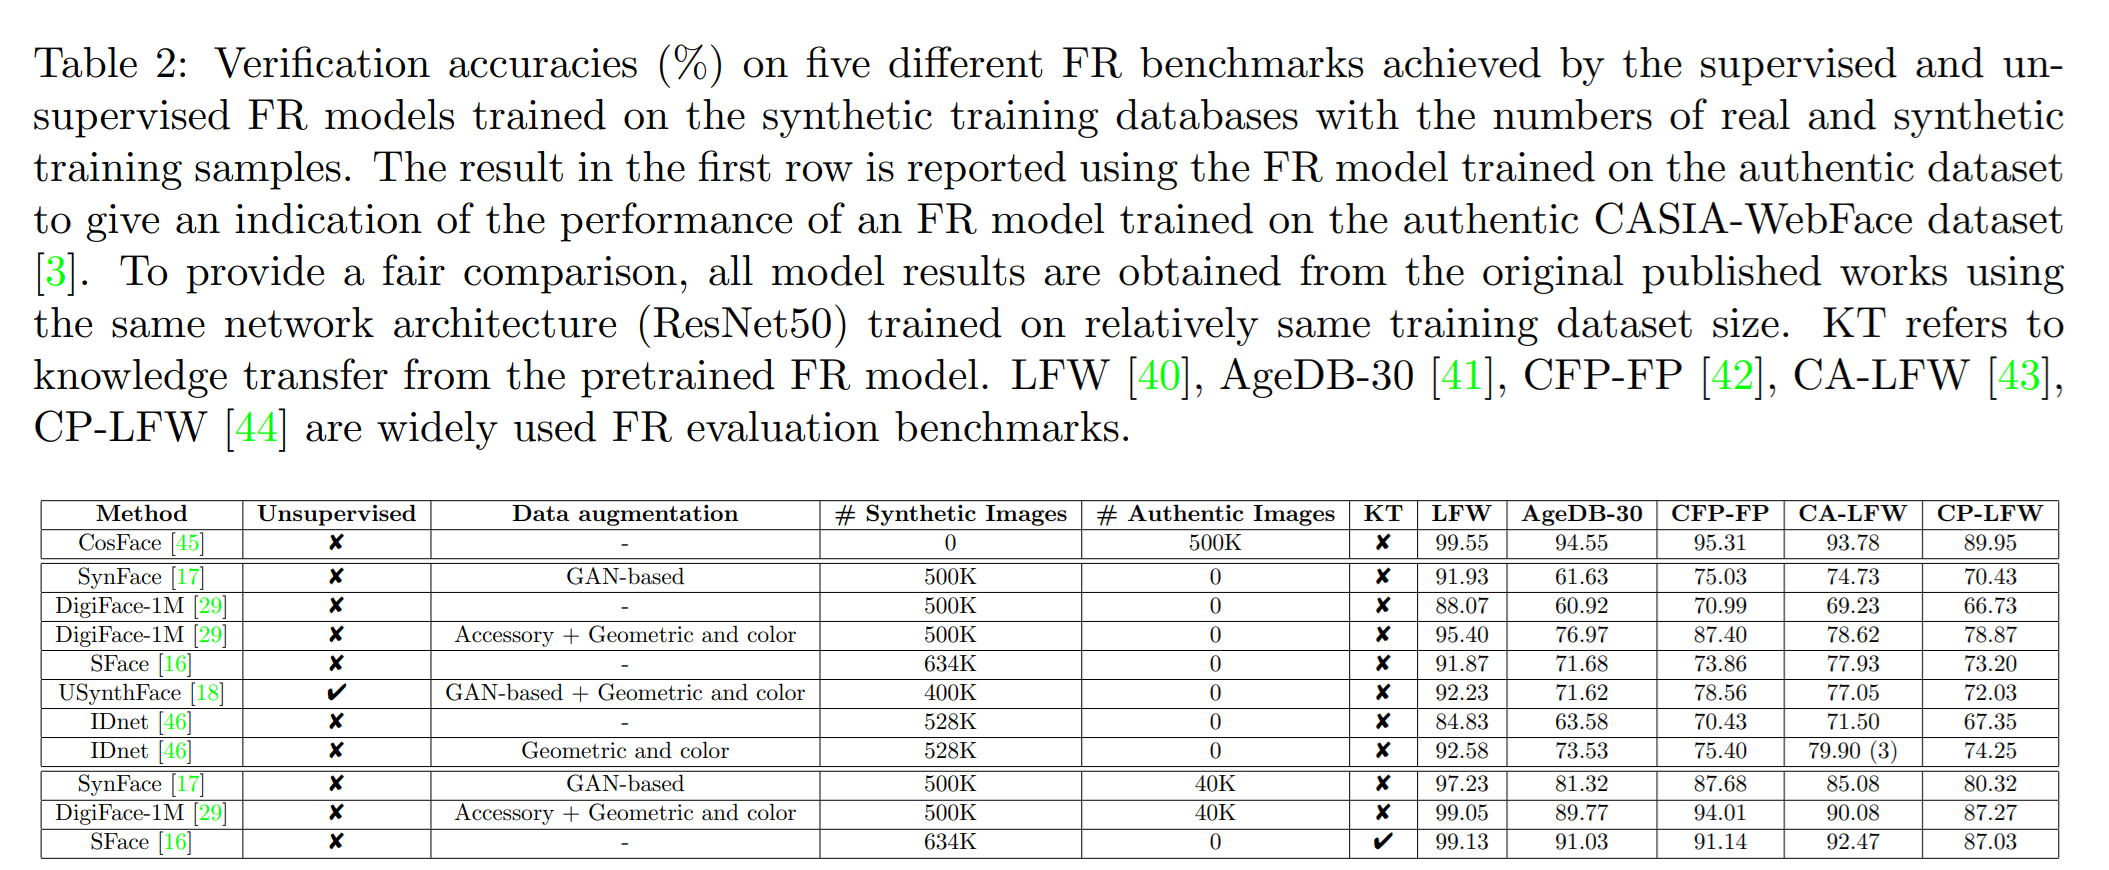
\includegraphics[scale = 0.6]{img3.png}
  \end{center}
  \item Evaluating FR:  SynFace presented a synthetic
  version of the Labeled Faces in the Wild (LFW)
  dataset and evaluated two FR models trained
  on authentic and synthetic data, respectively on the
  synthetic version of the LFW. The model trained on
  real data achieved an accuracy of 98.85\% and the
  one trained on synthetic data achieved an accuracy
  of 99.98\%. The work also suggested that the
  degradation in the verification performance between
  the two models is due to the domain gap between
  synthetic and real training images.
  \item Attacking FR: DGM approaches have been widely and successfully
  utilized to generate morphing, MasterFace, deepfake, and manipulation attacks on FR. Deep-fake and face manipulation
  attacks are already a serious problem facing modern societies and their generation is becoming more
  available and realistic with time.\\ Morphing attacks based on synthesized faces are a serious threat
  and FR recognition vulnerability to them is getting
  close to that of image-level morphing.\\ MasterFace attacks are relatively new, their initial proposed
  form is based on optimization on a relatively weak
  FR model with other works arguing their feasibility.
  \item Privacy Enhancement: 
  \begin{itemize}
    \item De-identification can be achieved by adding
    adversarial noise to the image, image obfuscation,
    and image synthesis, the latter being the core focus
    of this work. The main challenge so far
    in this domain is the cross-FR model performance as
    most works showed very good performances on the
    FR models that were used to optimize the solution,
    however, this performance drops when using other
    unknown FR models. 
    \item Syntheses-based soft-biometric
    privacy followed a similar trend as de-identification,
    however, with much less dominance in the literature. Here, as
    the target is the soft-biometrics and not the identity,
    the main challenge is to achieve generalized performance across soft-biometric estimators while maintaining FR performance across FR models.    
  \end{itemize}
\end{itemize}
\subsection{Future Prospects}
\begin{enumerate}
  \item Face Image Generation: Applications mainly require that
  the generated samples are of high visual fidelity with
  less focus on the identity information, which might
  be less optimal for biometric applications. When developing DGM for FR use-cases, the solution should
  focus on the utility of the generated images for the
  given tasks rather than only focusing on the humanperceived quality.
  \item Training FR: Research works target proposing network architectures or
  training paradigms designed specifically to learn from
  synthetic data. In general, training FR solutions of
  synthetic data still fails behind those trained on authentic data in terms of accuracy, which is the main
  practical shortcoming that hinders placing such solutions in practical use currently.
  \item Evaluating FR: The need for large-scale FR evaluation datasets that
  represent real scenario variations is the main motivation for future research directions on synthetic data
  for FR evaluation.
  \item Attacking FR: The constant struggle here is
  to always try to foresee new attacks and attack generation methodologies and analyze their strengths and
  weaknesses, leading to better mitigation strategies.
  \item Privacy Enhancement: The main challenge to generative face privacy enhancement is the generalizability and robustness as it
  must possess to maintain operation in real-world applications.
  \item Evaluation Protocols:  Much-needed set of evaluation
  metrics and protocols that can precisely and comparably answer the question of ``How well does the
  created data fit its targeted properties within its usecase?''. There is a need for
  such protocols and metric standards on the industrial level.
\end{enumerate}
\section{SynFace: Face Recognition with Synthetic Data}
Performance gap between the models
trained on real and synthetic face images can
be effectively narrowed by: 
\begin{enumerate}
  \item enlarging the intra-class variations via identity mixup
  \item leveraging a few real face images for domain adaption via domain mixup
\end{enumerate}
Discuss the impacts of synthetic datasets with different properties for face recognition, e.g., depth (the
number of samples per identity) and width (the number
of identities), and reveal that the width plays a more
important role. Analyze the influences of different facial attributes
on face recognition (e.g., facial pose, expression, and illumination).
\subsection{Terms}
\begin{itemize}
  \item Synthetic Data. Synthetic data for computer vision
  tasks has been widely explored, e.g., crowd counting,
  vehicle re-identification, semantic segmentation, 3D face reconstruction and face recognition. According to the motivation, existing methods can be categorized into three groups: (1) It is timeconsuming and expensive to collect and annotate large-scale
  training data; (2) It can be used to further improve the model trained on a real dataset; (3) It can
  be used to systematically analyze the impacts of different
  dataset attributes.
  \item Face Synthesis. With the great success of GANs, face synthesis has received increasing
  attention and several methods have been proposed to generate identity-preserving face images.
  \item Deep Face Recognition. Recent face recognition methods mainly focus on delivering novel loss functions for
  robust face recognition in the wild. The main idea is to
  maximize the inter-class variations and minimize the intraclass variations. 
  \item Mixup. Mixup uses the convex combinations of
  two data samples as a new sample for training, regularizing deep neural networks to favor a simple linear behavior in-between training samples. Vanilla mixup is usually
  employed on image pixels, while the generated data samples are not consistent with the real images, e.g., a mixup
  of two face images in the pixel level does not always form
  a proper new face image. 
\end{itemize}
\subsection{Method}
We first introduce deep face recognition
using margin-based softmax loss functions. We then explore the performance gap between the models trained on
synthetic and real datasets (SynFace and RealFace). Lastly,
we introduce (1) identity mixup to enlarge the intra-class
variations and (2) domain mixup to mitigate the domain gap
between synthetic and real faces images.
\subsubsection{Deep Face Recognition}
margin-based softmax loss
functions have been very popular in face recognition due to
their simplicity and excellent performance, which explicitly explore the margin penalty between inter- and intraclass variations via a reformulation of softmax-based loss
function. We use the cosine loss margin-based softmax loss.\\
To explore the performance gap between SynFace and
RealFace, as well as the underlying causes, we perform
experiments on real-world face datasets and synthetic face
datasets. We use CASIA-WebFace for
training and Syn-LFW for testing. We train two face recognition models on CASIA-WebFace and Syn 10K 50, and test them on
LFW and Syn-LFW, respectively. There is a clear performance gap (88.98\% vs. 99.18\%) when
testing on LFW, while SynFace outperforms RealFace on
Syn-LFW (99.98\% vs. 98.85\%).
\subsubsection{Identity Mixup}
To increase the intra-class variations of synthetic face
images, the Mixup Face Generator, which is capable of generating different identities and their intermediate states. 
\begin{itemize}
  \item Face Generator: It generates realistic face images $x$ from random noise $z$,
  which consists of five independent variables $z_i\in \mathbb{R}^{N_i}$ and
  each of them follows a standard normal distribution. The
  above five independent variables indicate independent factors for face generation: identity, expression, illumination,
  pose, and random noise accounting for other properties such
  as the background. The pipeline of
  generating a face image is to (1) first randomly sample latent variables from the standard normal distribution, (2) then
  feed them into the trained VAEs to obtain $\alpha, \beta, \gamma and \theta$ coefficients, and (3) the corresponding face image is synthesized
  by the generator using these coefficients.
  \item Identity Mixup: We propose to enlarge the intra-class variations by interpolating two different identities as a new intermediate one with changing the label correspondingly. We interpolate two different identity coefficient.\\
  The pipeline of Mixup Face
  Generator is first randomly sampling two different identity
  latent variables from the standard normal distribution, and
  then feeding them to the trained VAEs to obtain $\alpha_1,\alpha_2$ coefficients. The mixed identity coefficient $\alpha$ is obtained by
  identity mixup with $\alpha_1,\alpha_2$ by interpolation, the corresponding face image is finally synthesized by the generator.\\
  It is clear
  that the cyan triangles (Syn1) have the smallest variations
  , while the red circles (Syn3) have the largest one and the
  blue squares (Syn2) are in the middle position. Accordingly, the accuracy is in an increasing trend (i.e., 88.75\% $\rightarrow$
  89.47\% $\rightarrow$ 90.95\%). Both RealFace (trained on CASIA-WebFace) and SynFace IM (trained on Syn 10K 50 with identity mixup) are
  evaluated on five different synthetic testing datasets. R is interpolation coefficient. SynFace IM achieves nearly perfect accuracy when R is larger
  than 0.6, and also obtains an impressive 97.30\% result which remarkably outperforms the 87.83\% accuracy by RealFace when R is 0.6. On the other hand, the accuracy of
  RealFace drops significantly on Syn-LFW-R when R becomes small, which suggests that the domain gap between
  real and synthetic face data is still large even after employing the identity mixup.
  \begin{center}
    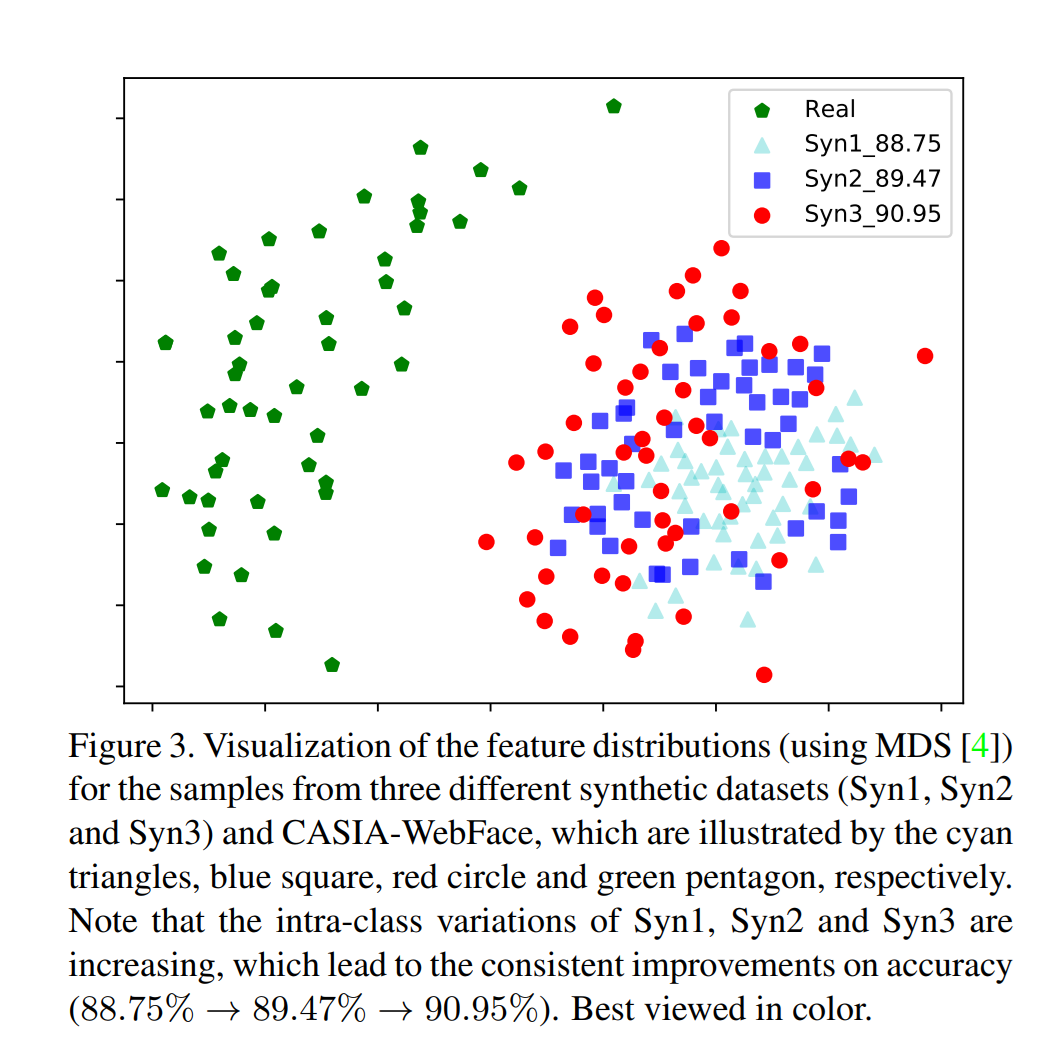
\includegraphics[scale = 1]{img4.png}
  \end{center}
  \item Domain Mixup: To further narrow the performance gap between
  SynFace and RealFace, we introduce the domain mixup as
  a general domain adaptation method to alleviate the domain
  gap for face recognition. Specifically, we utilize large-scale
  synthetic face images with a small number of real-world
  face images with labels as the training data. When training,
  we perform mixup within a mini-batch of synthetic images
  and a mini-batch of real images, where the labels changed
  accordingly as the supervision. For the large-scale synthetic data, we synthesize the
  Syn 10K 50 dataset that has 10K different identities with
  50 samples per identity. For a small set of real-world data,
  we utilize the first 2K identities of CASIA-WebFace.
  \begin{center}
    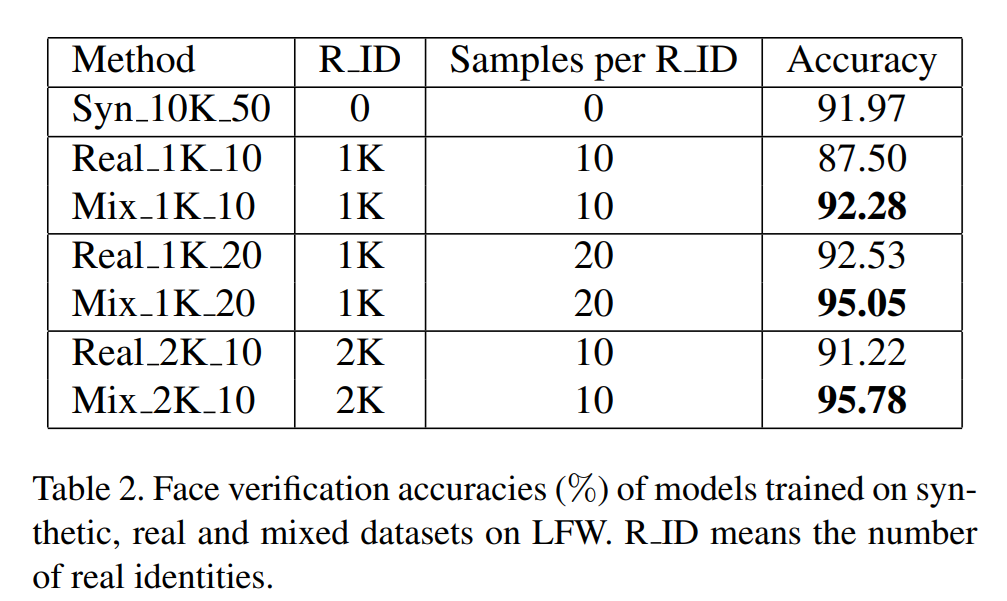
\includegraphics[scale = 1]{img5.png}
  \end{center}
  Domain mixup brings a significant and consistent improvement over the baseline methods under different settings.
\end{itemize}
\subsection{Experiments}
With the Mixup Face Generator, we are able
to generate large-scale face images with controllable facial
attributes, including the identity, pose, expression, illumination, and other dataset characteristics such as the depth
and the width.
\subsubsection{Datasets}
Real datasets: We employ the CASIA-WebFace
and LFW for training and testing, respectively.\\
\\
Synthetic datasets: We first generate a synthetic version of LFW, in which all synthetic face images share the
same properties with LFW images, e.g., expression, illumination, and pose. We then adopt the DiscoFaceGAN to generate the face
images according to these attribute coefficients with a random identity coefficient. Finally, we obtain a new dataset and refer to it as Syn-LFW, which has the same statistics
as LFW with unknown identities.\\
For
synthetic training dataset (e.g., Syn 10K 50), we construct
it by randomly sampling latent variables from the standard
normal distribution for identity, expression, pose and illumination coefficients, respectively, which leads to the same
person with different expressions, poses and illuminations
in the same class. 
\subsubsection{Implementation Details}
We use the MTCNN to detect face bounding boxes
and five facial landmarks (two eyes, nose and two mouth
corners). All face images are then cropped, aligned (similarity transformation), and resized to $112 \times 96$.
\subsubsection{Long-tailed Face Recognition}
Experimental Setup. To explore the long-tailed problem, we construct multiple synthetic datasets with the purpose that each dataset has the same number of identities
(2K) and total images (100K) but different degrees of unbalance. 
\begin{center}
  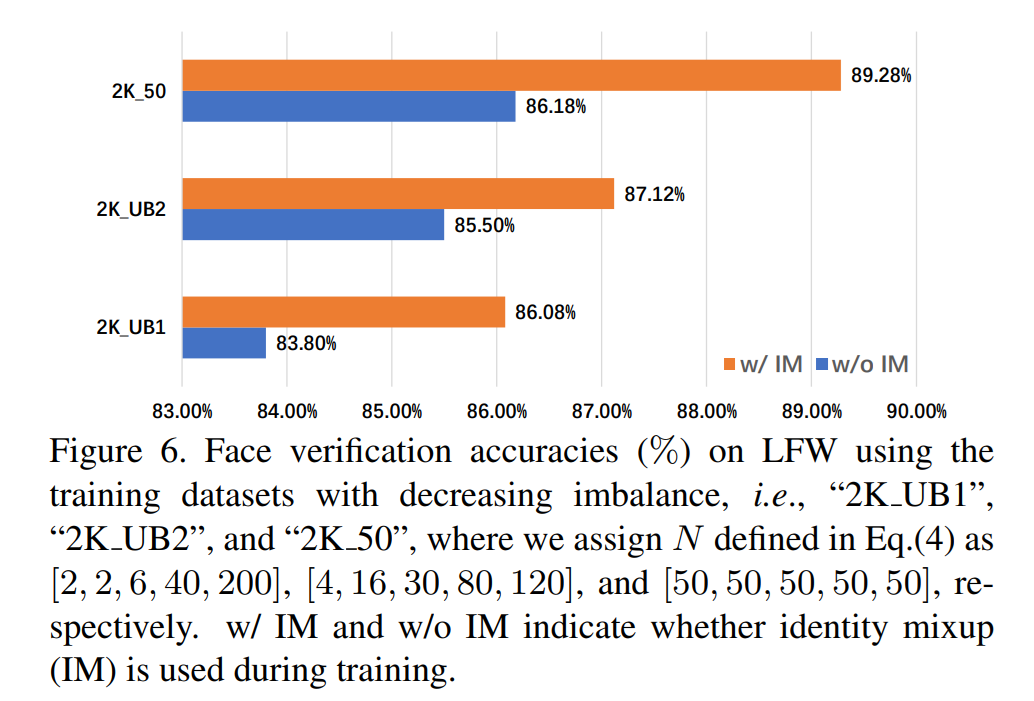
\includegraphics[scale = 1]{img6.png}
\end{center}
\subsubsection{Effectiveness of ``Depth'' and ``Width''}
Experimental Setup. We synthesize multiple face
datasets with different width (the number of identities) and
depth (the number of samples per identity). Let “N\_S” denote the synthetic dataset containing N identities with S
samples per identity.
\begin{center}
  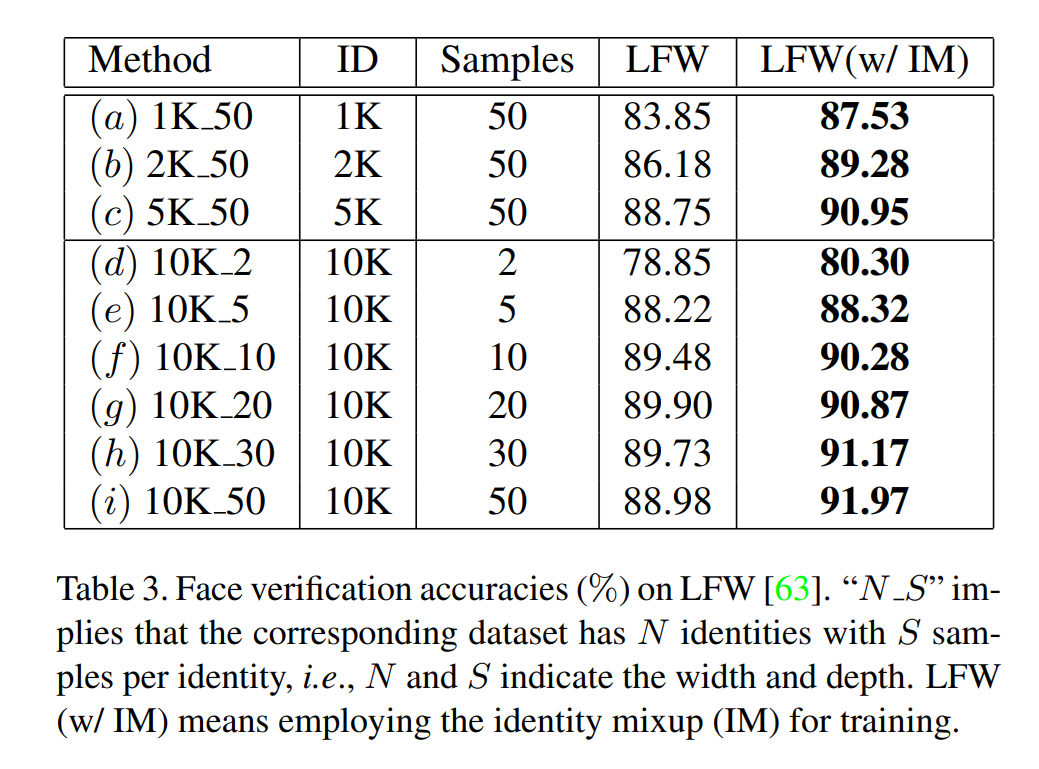
\includegraphics[scale = 1]{img7.png}
\end{center}
Firstly, we analyze the influence of the width of the dataset
by comparing the results of (a), (b), (c), (i). From (a)
to (c), we see that the accuracy dramatically increases from
83.85\% to 88.75\%. However, the improvement is marginal
from (c) to (i), which implies that the synthetic data may
suffer from the lack of inter-class variations. Observing the results of (d), (e), (f), (g), (h), (i), we conclude that
the accuracy significantly increases with the increasing of
dataset depth, but it is quickly saturated when the depth
is larger than 20.
\subsubsection{Influence of Facial Attributes}
Experimental Setup. We explore the impacts of different facial attributes for face recognition (i.e., expression,
pose and illumination) by controlling face generation process. We construct four synthetic datasets that have 5K
identities and 50 samples per identity. The difference between the four datasets is the distribution of different facial attributes.
\begin{center}
  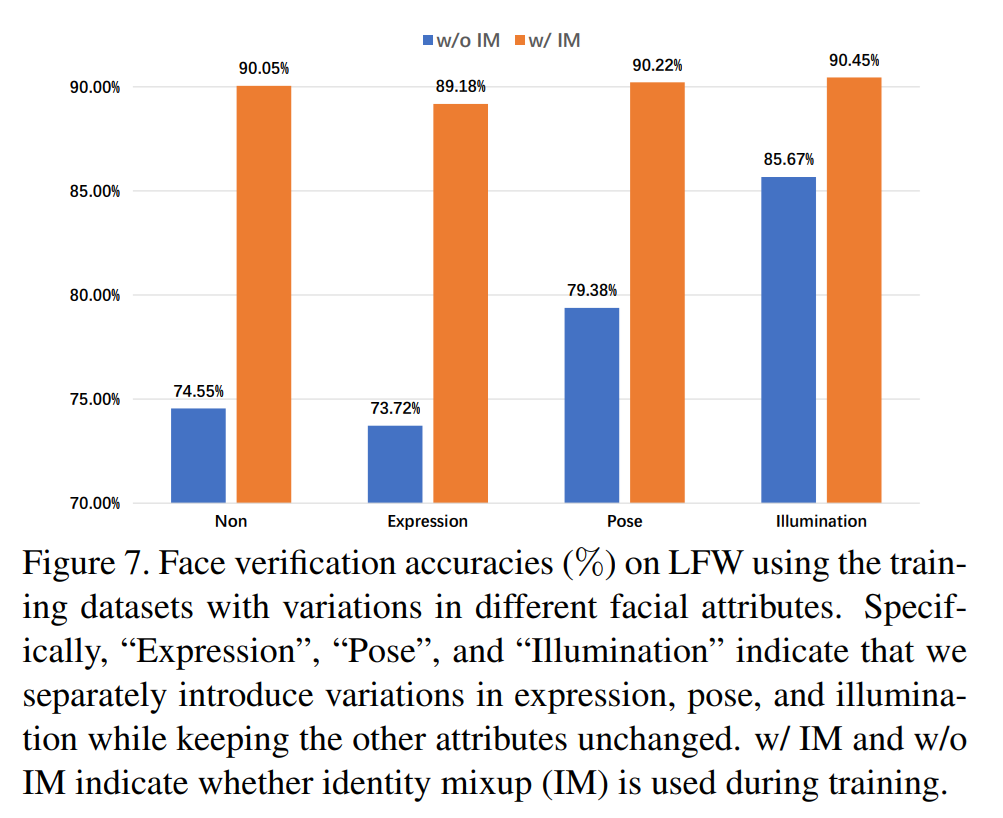
\includegraphics[scale = 1]{img8.png}
\end{center}
All of four
settings are significantly improved with the proposed identity mixup, especially for ``Non''. A possible reason is that
identity mixup can be regarded as a strong data augmentation method for face recognition, reducing the influences of
different facial attributes on the final recognition accuracy.
\section{On the Applicability of Synthetic Data for Face Recognition}
Analyses the differences between synthetically generated face images
and real face images from the biometric perspective. Face Quality Assessment Algorithms (FQAA)
quantify the biometric quality of a sample (for instance, face
image) by translating it to a quality score between [0, 100]. By measuring the face quality metrics of synthetically
generated face samples, we can establish if they can be
used for biometric algorithm training and testing purposes.
\subsection{Synthetic Face Image Generation and Dataset}
\subsubsection{Dataset}
Our synthetic data is generated
using StyleGAN and StyleGAN2 models which are
pre-trained on the FFHQ dataset. These generated images
are of resolution $1024 \times 1024$ pixels with high visual quality. To avoid variation, we truncate the latent space about the mean. To compare the synthetic data with real face data, we
chose a subset containing 24,025 images from the FRGCV2 face database as our representative dataset due to
relatively high-quality images and constrained conditions that
resemble the image quality in EES cases. To ensure that our
synthetic datasets have comparable conditions, we also discard
some unsatisfying images by having pre-selection criteria such
as minimum inter-eye distance (IED), illumination metrics
and predicted head poses to further improve the consistency
between our assessment and the facial quality requirements.
\subsubsection{Face Quality Assessment Algorithms}
\begin{enumerate}
  \item ISO/IEC 29794-5:2010 Implementation uses the handcrafted quality metrics. For each image under assessment, various hand-crafted
  quality metrics for facial images following the technical report
  ISO/IEC TR 29794-5 are extracted as a feature vector. Given
  the feature vector as an input, then a pre-trained Random
  Forest Regressor is applied to predict a quality score.
  \item FaceQnet v1 is a deep learning based FQAA and aims to predict the
  general utility of a face image, independent from a specific
  face recognition system. For the quality score prediction, a
  pre-trained network of ResNet-50 is fine-tuned on a small
  subset of VGGFace2 dataset including 300 data subjects. FaceQnet v1 follows a supervised learning approach, which
  means that the ground truth quality scores are required for
  fine-tuning the model. 
  \item SER-FIQ is an unsupervised
  technique that is not dependent on previously extracted ground
  truths in order to train the prediction model. Compared to
  FaceQnet v1, which outputs the general utility of a face image,
  SER-FIQ focuses on predicting the utility of a specific face
  recognition system. More precisely, the quality scores are
  based on the variations of face embeddings stemming from
  random subnetworks of a face recognition model. The main idea of SER-FIQ is to
add dropout layers as additional components to create random
subnetworks for each prediction of the same sample. Once
a fixed number of stochastic embeddings are extracted, the
sigmoid of the negative mean euclidean distances between
all embedding pairs is computed and outputs a quality score. 
\end{enumerate}
\subsection{Experiments and Results}
In order to compare the utility of face images from different
datasets, impostor distributions of comparison scores are created to evaluate differences in the similarity among non-mated
face images. The impostor distribution can show the diversity
of identity in each dataset and also can evaluate its verification
performance on FRS, in the circumstance that our synthetic
data is randomly generated without any mated samples. 
\subsubsection{Comparison between StyleGAN and StyleGAN2}
It is shown that the dataset generated with StyleGAN2 using a truncation factor of $\psi = 0.25$ has a higher
mean value of comparison score than StyleGAN. However,
this difference is reducing with the increase of $\psi$ and vanishes
as the truncation factor increases to 0.75. Similar to the impostor
scores, the distributions between StyleGAN and StyleGAN2
are close to identical across all FQAAs, thus reinforcing the
conclusion that StyleGAN and StyleGAN2 face images are
equally suitable for biometric recognition.
\subsubsection{Comparison between Synthetic and Real Data}
While
only 58\% of the StyleGAN2 images passed the filtering
pipeline, more FRGC images could be retained with a rate
of 75\%. The huge difference can be explained by the way
the data samples were acquired: StyleGAN2 is trained on
the FFHQ dataset, which has been webcrawled from a social media platform (Flickr). Both distributions have a
similar gaussian-curved shape with huge overlapping areas.
However, it is also visible that the right tail of the StyleGAN2
distribution is heavier compared to the FRGC dataset. In other
words, the similarity scores of non-mated comparisons are
slightly higher compared to those of FRGC, which potentially
causes higher False-Match-Rates.Looking at the FaceQnet v1 distributions,
both areas are nearly identical with a very low Kullback
Leibler Divergence of 0.111. However, steering the focus
on the SER-FIQ distributions, a clear shift in the peaks is
notable, which reveals that the estimated utility of the synthetic
images is lower compared to FRGC images. Several FRGC images
are annotated with high blurriness scores, which manifests
itself in a bimodal distribution. The reason for this observation
is due to the capturing process, where the images of multiple
subjects were captured in motion.
\begin{center}
  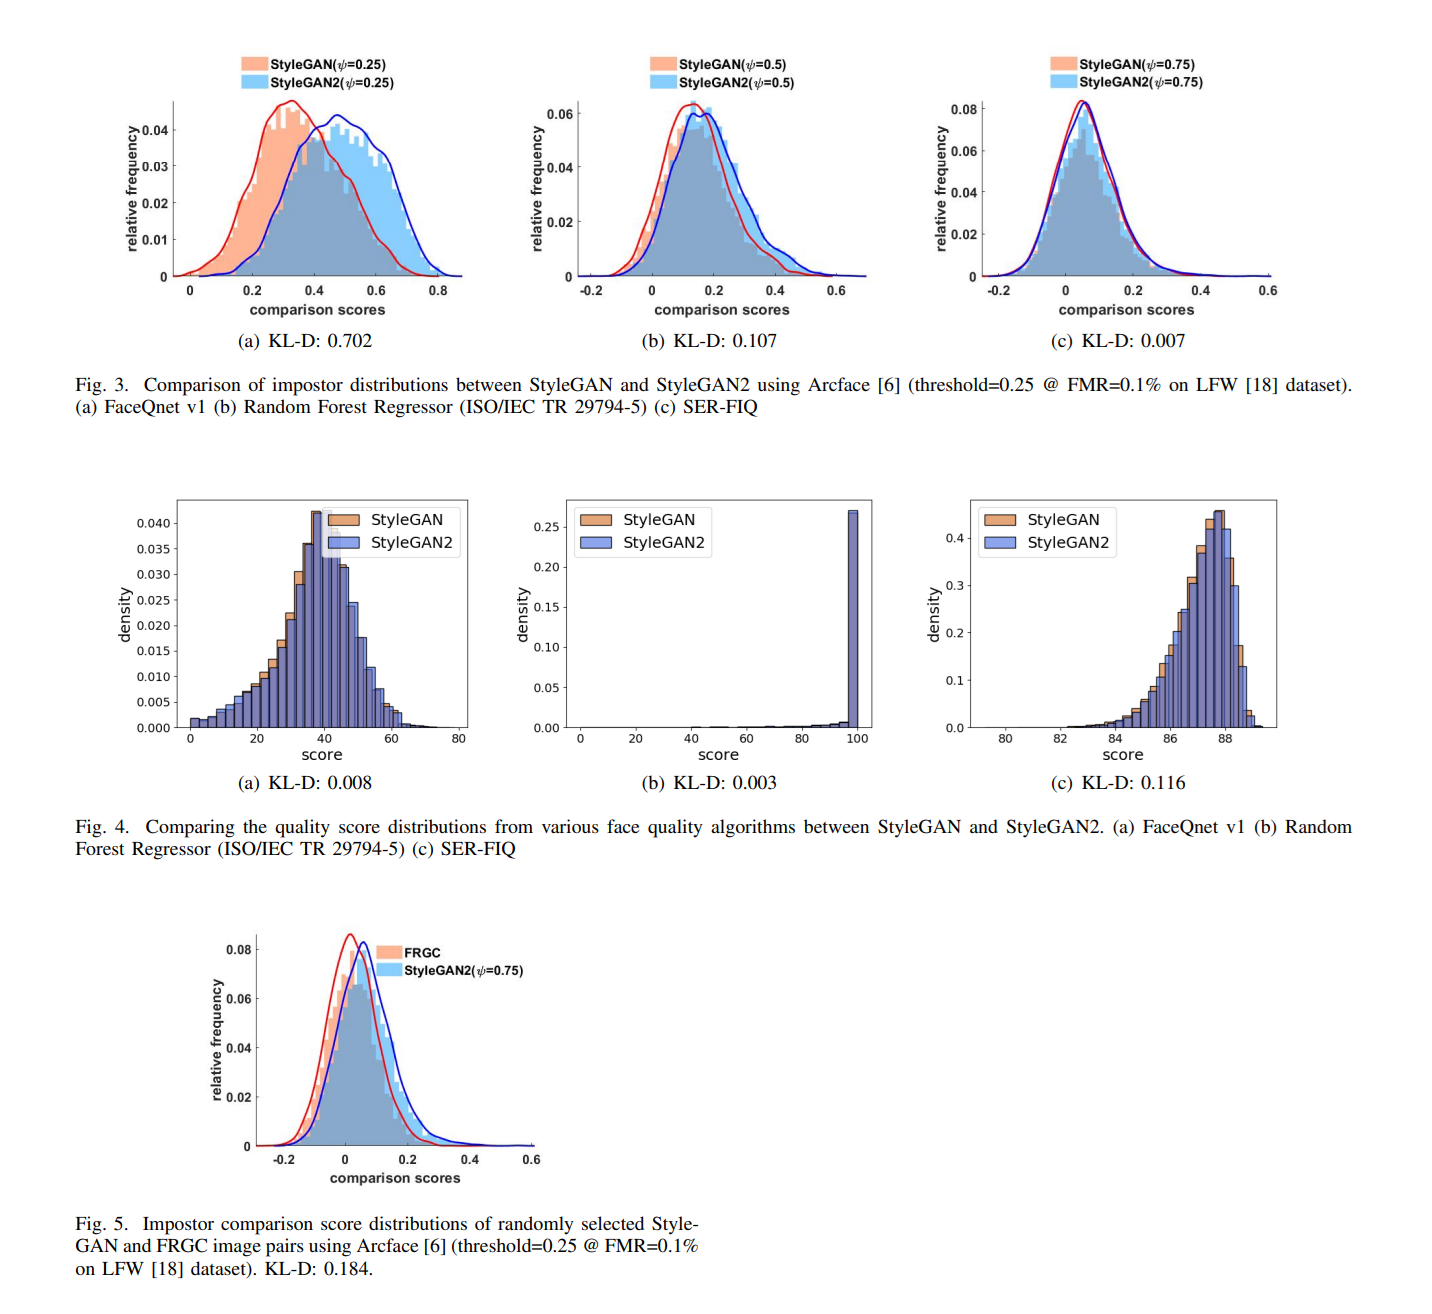
\includegraphics[scale = 0.9]{img9.png}
\end{center}
\section{Training Deep Face Recognition Systems with Synthetic Data}
\begin{itemize}
  \item A significant real-to-virtual performance gap exists between neural networks trained on synthetic and realworld data, which can be closed by fine-tuning with
  real-world data.
  \item Using synthetic data, we can either reduce the amount
  of real data needed to achieve competitive face recognition performance or combine it with large-scale real
  datasets to increase the recognition performance significantly across several standard benchmarks without
  database adaptation.
  \item Already good face recognition performances are
  achieved by using purely synthetic data, which is generated from just 200 real 3D scans.
  \item We did not observe any negative effects when pretraining with synthetic data, thus the performance gains
  come for free.
\end{itemize}
\subsection{Face Image Generator}
We propose to synthesize face images by sampling from a
statistical 3D Morphable Model of face shape, color and expression.
\begin{itemize}
  \item Facial identity. We assume that the facial identity is fully
  determined by the 3D face shape and color. We use the
  Basel Face Model 2017, for which the shape and color
  distribution is estimated from 200 neutral high-resolution 3D
  face scans. 
  \item Illumination. In our renderer, we assume the Lambertian
  reflectance model. We approximate the environment map with
  27 spherical harmonics coefficients (9 for each color channel).
  Sampling these coefficients randomly would lead to possibly
  unrealistic illumination conditions.
  \item Pose and Camera. The face is viewed by a fixed pinhole
  camera. The face orientation with respect to the camera is
  controlled by the six pose parameters (yaw, pitch, roll, and 3D
  translation). 
  \item Background. We simulate changes in the background with a
  non-parametric background model by sampling randomly from
  a set of background images of the describable texture database. The synthesized images are fully specified by the aforementioned parameter distributions which were lear-ned from
  a population of 3D face scans.
  \item Software. The face image generator was created with the
  scalismo-faces library
  and is publicly available. It is based
  on our previous work where we used a simple point light
  source and a discrete sampling of the parameters to study
  the influence of nuisance transformations on face recognition
  systems in the virtual domain.
\end{itemize}
\subsection{Experiments}
\subsubsection{Setup}
All experiments are based on the OpenFace framework, as the software is publicly available and well documented.
For the face detection and alignment we use an implementation
of the Multi-task CNN.\\
Real-world training and benchmark data. Whenever we
train a network with real-world data, the data is sampled
from the cleaned Casia WebFace dataset [41], which comprises 455,594 images of 10,575 different identities. From this
dataset, we remove the 27 identities which overlap with the
IJB-A dataset.\\
For bench marking, we use:
\begin{enumerate}
  \item CMU-Multipie
  \item LFW
  \item IJB-A
\end{enumerate}
Synthetic face image generation setup. The synthetic face
images are generated by randomly sampling the parameters of
our face image generator. Our synthetic dataset
consists of 1 Million images with 10K different identities and 100 example images per identity. The head pose is randomly sampled according to a uniform pose distribution on the yaw, pitch
and roll angles in the respective ranges $r_{yaw} =$ [-90, 90], $r_pitch = $[-30, 30] and $r_{roll}$ = [-15, 15].\\
Evaluation protocol. We evaluate face recognition networks at
the task of face verification. Thereby, we measure the distance
between two face images as the cosine distance between their
128-dimensional feature embeddings from the last layer of the
FaceNet model. For comparing the templates in the IJB-A dataset, we perform
softmax averaging of the similarity scores between each image.
\subsubsection{The real-to-virtual gap in face recognition}
We train a FaceNet-NN4 model with the Casia
dataset (referred to as FaceNet-Casia) and the synthetically
generated SYN-1M data (referred to as FaceNet-Synth). On the CMU-Multipie benchmark (Fig. 2a), both networks perform similarly, suggesting that 3DMMs can very well model
the facial appearance variation in a controlled setting. Whereas
in the more challenging settings of LFW (Fig. 2b) and IJBA (Fig. 2c) the FaceNet-Synth model performs significantly
worse than FaceNet-Casia. Hence, a prominent real-to-virtual
gap can be observed.
\subsubsection{Closing the real-to-virtual gap}
We fine-tune the FaceNetSynth model with real-world data. we randomly sample subsets of
the Casia dataset with size N = $\{10K, 50K, 100K, 200K\}$.\\
General observations. We can observe the following general effects: (1) Fine-tuning FaceNet-Synth with any amount of
real data leads to an increase of the recognition performance
compared to the original FaceNet-Synth and thus reduces the
real-to-virtual gap. (2) The size of the realistic dataset used
for fine-tuning positively correlates with the final recognition
performance. (3) With a subset of only 100 - 200K images,
the real-to-virtual gap is closed and the fine-tuned network outperforms FaceNet-Casia on all benchmarks. (4) Using the full
Casia dataset for fine-tuning even increases the performance
gain\\
Benchmark-specific observations: On the LFW dataset the real-to-virtual gap can be almost closed with
100K realistic training examples. Thus, pre-training on synthetic data reduced the amount of data needed to achieve
similar performance as FaceNet-Casia by about a factor of
five. For the IJB-A dataset  100K images do not suffice
to close the real-to-virtual gap. When finetuning with 200K images, we achieve a significantly improved
performance compared to the FaceNet-Casia network.
\begin{center}
  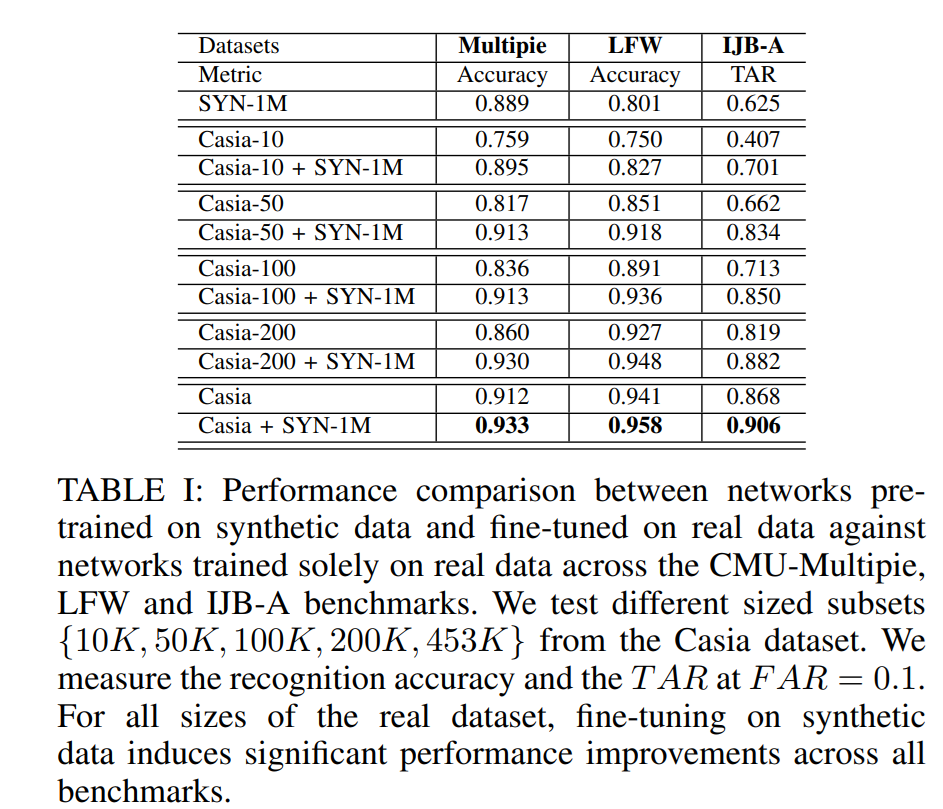
\includegraphics[scale = 1]{img10.png}
\end{center}
Pre-training on synthetic data always increases the performance compared to training with real data only. For the small
50K subset the performance increase is very prominent and
already results in highly competitive performances. Notably,
pre-training on synthetic data leads to a performance increase
across all benchmarks, even though the benchmarks have very
different imaging characteristics.
\subsubsection{Changing the characteristics of the synthetic dataset}
We change one dataset characteristic at a time while keeping all other parameters of our data generator fixed.\\
\\
Bias to frontal pose. We generate the SYN-1M-Front
dataset which, compared to the SYN-1M dataset, is limited
in the yaw angle to the range of $r_{yaw} =$ [-35, 35]. With
this setup, we simulate a bias towards frontal head poses,
which is prevalent in many datasets. Training the FaceNetNN4 architecture with the SYN-1M-Front data induces a significant performance decrease compared the SYN-1M dataset,
in which the pose distribution varies across the full yaw angle. The performance decrease is also present after finetuning on the Casia dataset.\\
Increasing the number of training identities. In this setup,
we double the number of identities to 20K, thus generating
two million synthetic training images.The network trained solely on the SYN-2M
dataset performs slightly worse than with the SYN-1M data,
which might be due to some overfitting to the synthetic domain. However, after fine-tuning an increase in the recognition
performance can be observed.
\begin{center}
  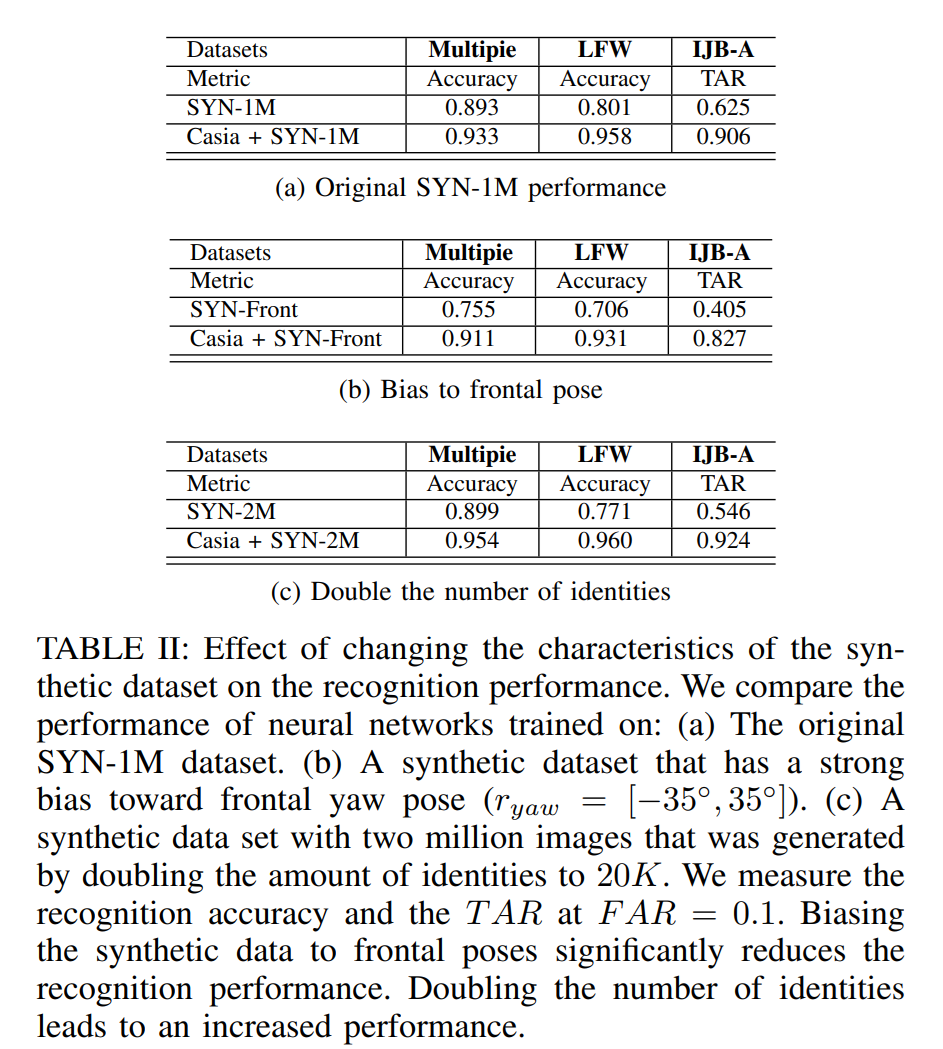
\includegraphics[scale = 1]{img11.png}
\end{center}
\section{Unsupervised Face Recognition using Unlabeled Synthetic Data}
\subsection{Methodology}
\subsubsection{Unsupervised Face Recognition}
\begin{itemize}
  \item Unsupervised representation learning: It uses contrastive learning to maximize the similarity between feature representations of positive pairs and minimize the similarity between feature representations of negative
  pairs. Consider a query image $q$ encoded into $f_q$, a positive key
  of the same instance of $q$, augmented as $k^+$ and encoded into
  $f_{k^+}$ along with a set of negative keys $\{k^-_i\}^K_{i=1}$ (encoded into
  $\{f_{k^-_i}\}^K_{i=1}$) that are retrieved from the queue. A contrastive
  loss that guides the model to enhance the similarity between $f_q$ and $f_{k^+}$ to be larger than the similarity between $f_q$
  and $\{f_{k^-_i}\}^K_{i=1}$ can be measured using MarginNCE as
  follows:
  \[L=-\log\dfrac{exp((f_q\times f_{k^+}-m)/\tau)}{exp((f_q\times f_{k^+}-m)/\tau)+\sum_{i=1}^{K}exp((f_q\times f_{k^-_i})/\tau)}\]
  \begin{center}
    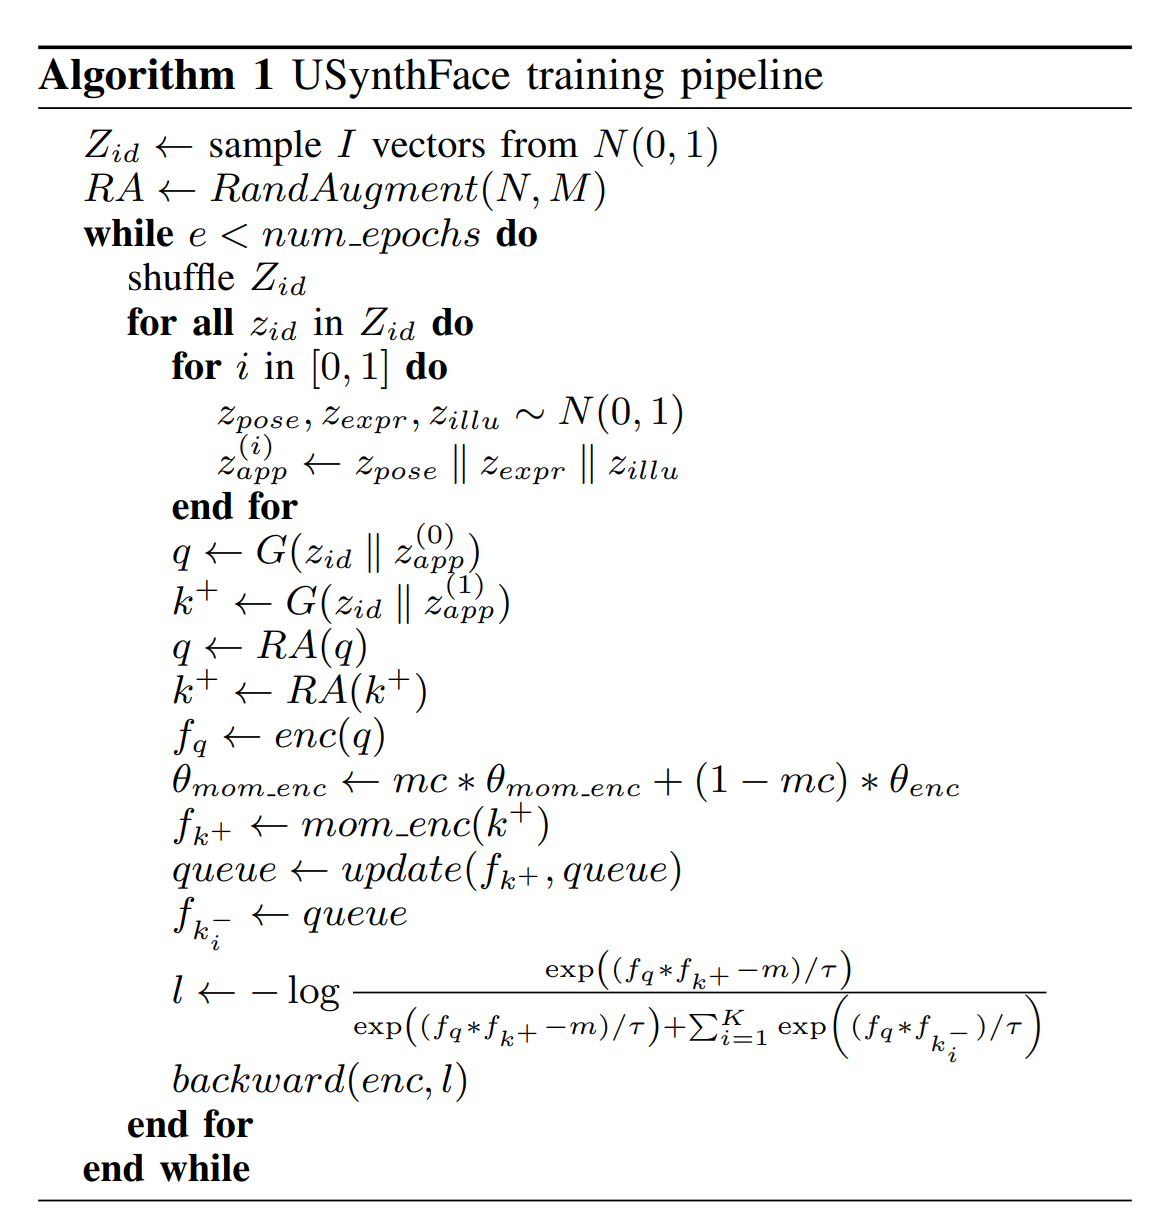
\includegraphics[scale = 0.8]{img12.png}
  \end{center}
  \item  Synthetic data generation: We used DiscoFaceGAN (DFG) to conditionally generate I images with different identity, pose, illumination,
  and expression. DFG presented a 3D morphable face model
  (3DMM) to the StyleGAN model, enabling disentanglement of identity, pose, expression and illumination in the
  latent space to conditionally generate realistic images with
  varying attributes.
  \item Data augmentation: We propose to enrich the conventional data augmentation
  operations, i.e. geometric and color transformations with
  GAN-based augmentations generated by a conditional generative model. The conventional data augmentation method
  is based on RandAugment. Two augmented views of the
  same image (and thus identity) can be generated by fixing
  the identity latent and randomly modifying the attribute
  latent vectors.
\end{itemize}
\subsection{Setups}
\subsubsection{Datasets}
\begin{itemize}
  \item Training: A DFG-model is trained on Flickr-FacesHQ dataset (FFHQ) that contains 70k images of the size
  $1024\times1024$ pixels collected from Flickr and encompass variation in ethnicity, age, image background, and accessories. We opt to generate 100K images from the DFG model,
  each from different identity latent representations.
  \item Evaluation: We used in this paper the
  following datasets as evaluation benchmarks for our ablation
  studies: Labeled Faces in the Wild (LFW), AgeDB30, Celebrities in Frontal to Profile in the Wild (CFPFP), Cross-Age LFW (CA-LFW), and CrossPose LFW (CP-LFW). The verification accuracy is
  reported for each of the considered benchmarks following
  their defined protocols.
\end{itemize}
\subsubsection{Implementation Details}
ResNet-50 architecture. Temperature = 0.07. Queue size = 32768. SGD with LR = 0.1. The momentum is set to 0.9 and
the weight decay to 5e-4. The learning rate is divided by
10 after 8, 16, 24, and 32 epochs.
\subsection{Results}
\subsubsection{ To which degree does data augmentation effect identity
information?}
The two augmented versions of
the same image (instance) were considered as a genuine pair
and pairing with any other image of different instances is
considered as an imposter pair. We used SOTA FR model
ElasticFace (ElasticFace-Arc) to extract representation
features of our synthetic data. The achieved verification
performances are reported as Equal Error Rate (EER),
FMR10, FMR100, and FMR1000, which are the lowest
false non-match rate (FNMR) for a false match rate (FMR)
$\leq$10.0\%, $\leq$1.0\% and $\leq$0.1\% respectively, along with plotting the genuine-imposter score distributions. (1) GAN-based augmentations (pose,
illumination and expression) preserve to large degree the
identity information of the augmented sample (0.0110 EER). (2) Color and geometric
transformations through RandAugment lead to degradation
in verification performance (0.0967 EER) in comparison to
GAN-based augmentation. (3) As expected, combining GANbased with RandAugment achieve the lowest verification
performance (0.1650 EER) in comparison to the GAN-based
(0.0110 EER) and RandAugment (0.0967 EER).
\subsubsection{Does the synthetic data share identity information with
the GAN authentic training data?}
We answered this question
by conducting an N:N evaluation where references were
compared to probes from the GAN authentic training dataset
(noted as R-R) and N:M evaluation where authentic references from the GAN training dataset were compared
to synthetic probes generated by GAN generator model
(noted as R-S). R-R and R-S score distributions are highly overlapped and
only a few samples are considered matched, i.e. achieved
comparison scores higher than the operational threshold.
\subsubsection{Impact of GAN-based augmentation}
We evaluated the impact of GAN-based augmentation
on our USynthFace by training and evaluating USynthFace
model with widely used augmentation operation in FR horizontal-flipping. This model is considered
as a baseline in this study. Then, we trained a second instance
of the baseline model with GAN-based augmentation, i.e.
pose, illumination and expression (in addition to horizontalflipping). One can clearly notice that including GAN-based augmentation in the model training significantly improved the
verification accuracies in comparison to the baseline model.
\subsubsection{Impact of conventional data augmentation}
The candidate operation is included in the final augmentation space if it
has led to improvement in overall verification performances
(in terms of Borda count) in comparison to the baseline
model. Out of 15 candidate operations, 12 operations outperformed the baseline operation. These operations are included
in the search space of RandAugment.
\subsubsection{Conventional data augmentation through RandAugment}
The augmentation operations from the previous study are used to build the search space for
RandAugment. We evaluate in this section by randomly
augmenting the training samples with multiple operations,
i.e. 1, 2, 3 or 4 and with different magnitudes, i.e. 8,
12, 16, 20 or 24. In total, we trained and evaluated 20
models (4 different numbers of operations and five possible
magnitudes). The best verification performance is achieved
by randomly applying 4 operations (sequentially) with the
magnitude of 16.
\subsubsection{Analyses of the queue size}
Maintaining a queue of 32768 negative keys leads to the highest overall
verification performance on the considered evaluation benchmarks. 
\subsubsection{Study of feature representation dimensionality}
Best overall verification performance is achieved using feature
representation of 512-D.
\subsubsection{Training optimization}
To provide complete evaluation results, we
study increasing the number of epochs to a maximum of
200 [10] and using a plateau-based learning scheduler. The
initial learning rate is set to 0.1 and it divided by 10 when
the average validation accuracy does not improve for 10
consecutive epochs. The training is stopped when the average
validation accuracy does not improve for 20 consecutive
epochs with maximum of 200 epochs. Increasing the training epochs
significantly improved the verification performance on all
considered benchmarks.
\subsubsection{Impact of different margins in MarginNCE}
Vverall verification performance
is improved by increasing margin values from 0 to 0.1.
However, when we increase the margin value to 0.15 or 0.20,
the overall verification performances are slightly degraded.
\subsubsection{Study of training database size}
SynFace and SFace are trained with supervised learning to learn
multi-class classification using margin-penalty softmax loss.
SynFace only reported the verification performance on LFW
dataset. On LFW and CFP-FP datasets, our unsupervised
model outperformed SFace and SynFace. On AgeDB-30,
CA-LFW and CP-LFW, our unsupervised model achieved
very competitive results to SFace, even though USynthFace
training is unsupervised.
\section{Face Recognition: Too Bias, or Not Too Bias?}
\subsection{The BFW Benchmark and Dataset}
\subsubsection{Data}
Data is made up of evenly split subgroups, but with an increase in subgroups (i.e., IF and IM), subjects per subgroup, and face pairs.
\begin{itemize}
  \item Compiling subject list. Subjects were sampled
  from VGG2 - unlike others built from multiple sources, BFW has fewer potential conflicts in
  train and test overlap with existing models. To
  find candidates for the different subgroups, we first
  parsed the list of names using a pre-trained ethnicity model.
  \item Detecting faces. Faces were detected using
  MTCNN. Then, faces were assigned to one
  of two sets. Faces within detected bounding box. (BB) regions extended out 130\% in each direction,
  with zero-padding as the boundary condition madeup one set. The second set were faces aligned and
  cropped for Sphereface.
  \item Validating labels. Faces of BFW were encoded
  using the original implementation of the SOTA
  Sphereface. For this, each face was aligned to
  predefined eye locations via an affine transformation. Then, faces were fed through the CNN twice
  (i.e., The original and horizontally flipped), with
  two features fused by average pooling. the median (i.e., 50 percentile) of all scores for a face with respect to all of
  faces for the respective subject must pass a threshold of $\theta$ = 0.2; else, the face is dropped.
  \item the median (i.e., 50 percentile) of all scores for a face with respect to all of
faces for the respective subject must pass a threshold of $\theta$ = 0.2; else, the face is dropped.
\end{itemize}
Face recognition:
\[f_{boolean}(\vec{x}_i,\vec{x}_j) = d(\vec{x}_i,\vec{x}_j)\leq \theta\]
\subsubsection{Human Assessment}
To focus on the human evaluation experiment,
we honed-in on pairs from two groups, White
Americans (W) and Chinese from China (C). there were 60 W and 60 C,
both with Male (M) and Female (F) split evenly. A
total of 50 face pairs of non-famous “look-alikes”
were collected from the internet, with 20 (WA) and
20 (C) pairs with, again, M and F split evenly. The
other 10 were of a different demographic (e.g., Hispanic/ Latino, Japanese, African). 
\subsection{Results and Analysis}
LFW has about 13\%, 14\%, 3\%, and 70\% ratio in
Asian, Black, Indian, and White, respectively. Furthermore, CASIA-Web is even more unbalanced
(again, as reported in [38]), with about 3\%, 11\%,
2\%, and 85\% for the same subgroups.
\begin{itemize}
  \item DET analysis. DET curves (5-fold, averaged)
  show per-subgroup trade-offs. M performs better than F, precisely as one would
  expect from the tails of score-distributions for genuine pair. AF and IF perform the worst.
  \item Score distributions for imposters
  tend to peak about zero for all subgroups, and with
  minimal deviation comparing modes of the different plots. On the other hand, the score distribution of the genuine pairs varies across subgroups in
  location (i.e., score value) and spread. A vast majority of errors occur in the
  intra-subgroup. It is interesting to note that while
  the definition of each group based on ethnicity and
  race may not be crisply defined, the confusion matrix indicates that in practice, the CNN finds that
  the groups are effectively separate. The categories
  are, therefore, meaningful for FR.
  \begin{center}
    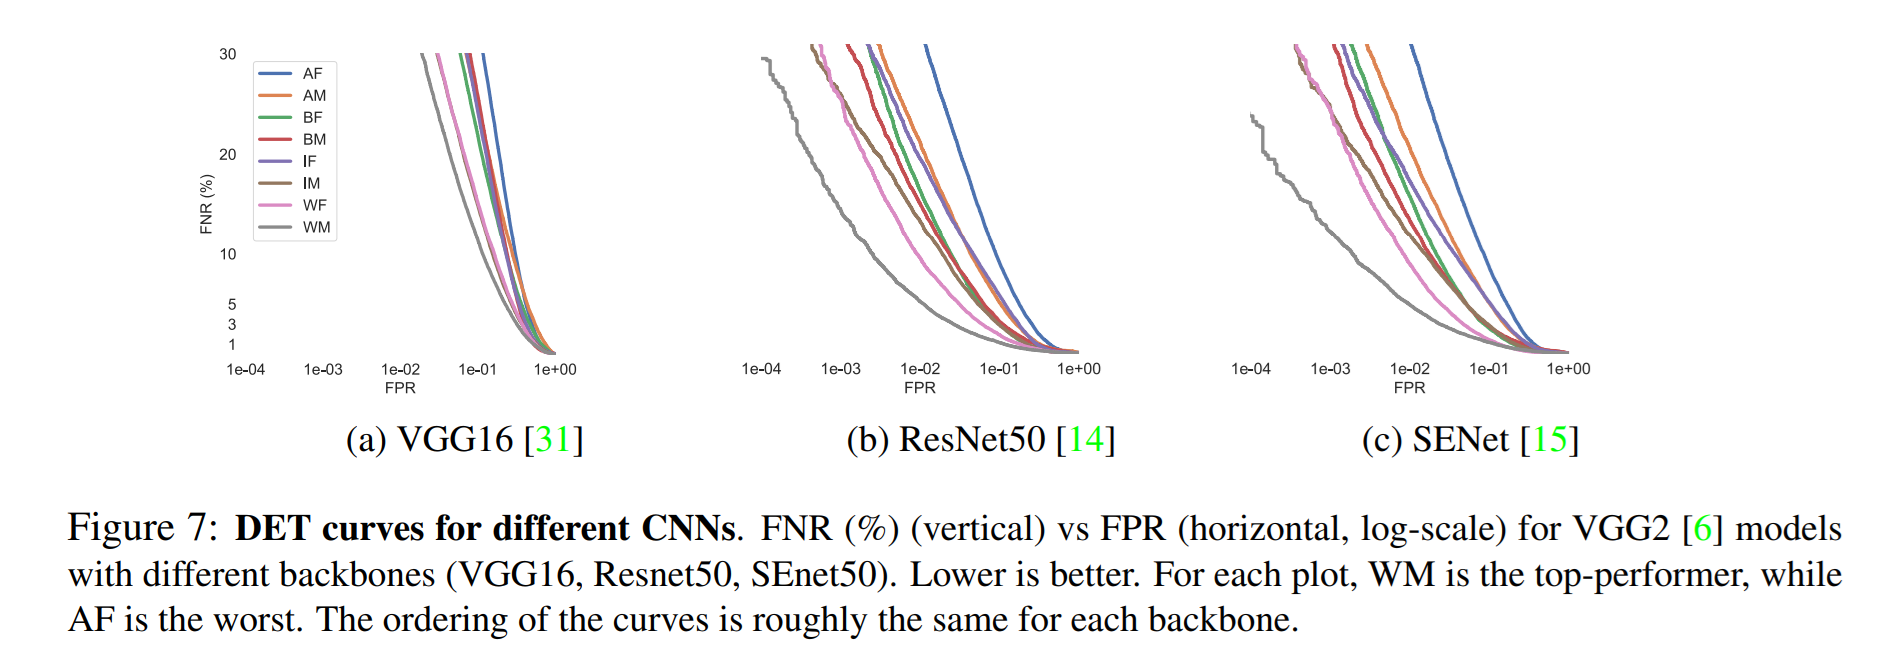
\includegraphics[scale = 0.7]{img13.png}
  \end{center}
  \item Model Analysis: Similar trends across
  subgroups and models, which is consistent with
  Sphereface as well. For example, the plots
  generated with Sphereface and VggFace2 all have
  the WM curve at the bottom (i.e., best) and AF on
  top (i.e., worst). Thus, the additional CNN-based
  models demonstrate the same phenomena: proportional to the overall model performance, exact in
  the ordering of curves for each subgroup.
  \item Verification threshold analysis. We seek to reduce the bias between subgroups. Such that an
  operating point (i.e., FPR) is constant across subgroups. Even for lower FAR, there are notable improvements, often of the order of 1\%, which can be challenging to achieve when FAR is near $\geq$90\%. More
  importantly, each subgroup has the desired FPR,
  so that substantial differences in FPR will remain
  unfounded. 
  \item Human Evaluation Analysis:  Each subgroup is best at labeling their type, and then second best at labeling
  the same ethnicity but opposite sex. Performance on BFW improved with subgroup-specific thresholds.  as the recognition performances drop with a global threshold optimized for
  one subgroup and deployed on another, human performance tends to fall when across subgroups.  
\end{itemize}
\section{Mitigating Demographic Bias in Face Recognition via
Regularized Score Calibration}
\begin{itemize}
  \item We propose a regularization-based approach to mitigate demographic bias in FR systems by incorporating
  score normalization-based regularization term.
  \item Unlike many bias mitigation methods, our method
  does not require a separate classifier or additional
  computational resources, making it more efficient and
  practical for deployment.
  \item With the intra- and inter-demographic regularization
  terms, our work focuses on improving both aspects of
  fairness - whereas many existing bias mitigation
  works solely focus on the latter.
  \item We evaluated performance of the proposed regularization method on three datasets and three backbone FR CNNs for in- and cross-dataset setups. Our experimental results demonstrate improvement in demographic
  fairness, without compromising recognition accuracy.
\end{itemize}
\subsection{Bias Mitigation via Regularization}
\subsubsection{Training Regular FR CNN}
The training
procedure often considers FR as a classification problem
where the subject's identity label acts as the ground truth
or target, and a suitable classification loss function, $\mathcal{L}_{cls}$, is
minimized via Stochastic Gradient Descend (SGD). 
Most state-of-the-art FR systems employ an extension of typical cross-entropy loss such as ArcFace,
SphereFace, ElasticFace, etc.
\subsubsection{Demographic Calibration for Fairnes}
Given an FR CNN
$f(., \theta)$, we hypothesize that the possible causes of demographic biases are:
\begin{enumerate}
  \item the distribution of f(matching scores) for some demographic groups might exhibit a multi-modal behaviour (one would ideally expect a bi-modal distribution: one for mated scores and another for non-mated ones).
  \item Non-alignment of distribution of matching scores of different demographic groups.
\end{enumerate} 
We use the platt loss function:
\[\mathcal{L}_{intra-d}(f(x_j), f(x_k), z_{jk})=z_{jk}\log g(f(x_j),f(x_k))+(1-z_{jk})\log (1-g(f(x_j),f(x_k)))\]
While this loss term, by clustering scores, has improved the
recognition performance of each demographic group separately, we would still require different score thresholds for
each demographic group for optimal classification. The use
of such thresholds requires accurate knowledge of demographic label of each sample at run-time. We propose to incorporate an inter-demographic loss component which penalizes large differences between intrademographic loss values of different demographic groups. Finally we get:
\[\theta^*,\psi^*=\underset{\theta,\psi}{argmax}\dfrac{1}{N}\sum_{i=1}^N\left[\mathcal{L}_{cls}(f(x_i,\theta);y_i)+\lambda_{inter-d}\mathcal{L}_{inter-d}(\left[\psi_1,\ldots,\psi_D\right])+\right.\]
\[\left.\lambda_{intra-d}\sum_{d=1}^D\mathcal{L}_{intra-d}(f(x_j , \theta), f(x_k, \theta), z_{jk}, d_{jk})\right]\]
\subsection{Experimental Results}
\subsubsection{Datasets}
Datasets: For our experimental analysis of the demographic regularization method, we utilized three publicly
available FR datasets that provide race or ethnicity information: VGGFace2, MORPH, RFW
\begin{itemize}
  \item FR CNN Backbones: We worked with the FR CNN based
  on the iResNet architecture with either 34, 50, or 100 layers. These models were trained using ArcFace loss on
  the MS1MV3 dataset, which is a refined version of the MSCeleb1M dataset.
  \item FR Pipeline: For consistent experiments, each combination of dataset and backbone underwent a standardized preprocessing procedure. This involved using MTCNN for initial face detection and facial landmark identification. The
  resulting 5 landmarks were then used to align and resize the
  face region to meet the specified requirement of $112 \times 112$
  pixels, as required by each iResNet-based FR CNN architecture. 
  \item Performance Evaluation: To measure recognition accuracy, we determined the score threshold on the train set considering the Equal Error Rate (EER). This threshold was
  then used to convert scores from the test set into binary
  decisions. Alongside recognition accuracy, we also report
  false accept rate and false reject rate for the test set, which
  indicate misclassifications of imposters and genuine samples respectively.
\end{itemize}
\subsubsection{Results of regularization experiment}
\begin{itemize}
  \item Results on VGGFace2:Overall recognition accuracy increased by 0.63\%, 0.12\%, and 0.33\% respectively
  for FR CNNs with 34, 50, and 100 layers after proposed
  regularization. There were slight improvements in accuracy for almost each demographic group for the proposed
  method. At the same time, the variation in recognition accuracy among different demographics decreased as indicated
  by the reduced standard deviation (std) and skewed error
  rate (SER) metrics. For each demographic's scores are better aligned in regularized cases, especially for 50- and 100-layer FR backbones.\\
  During the evaluation of the same FR CNN on the RFW dataset, we noticed a substantial decrease in accuracy
  and fairness metrics compared to the baseline performance.\\
  The performance of three FR CNNs improved when
trained with balanced settings on the RFW dataset. For
both backbones, 50- and 100-layered iResNets, the overall
accuracy increased by nearly 1\%, while reducing the standard deviation by 25\% compared to the respective baseline
numbers. Although there were not consistent improvements
in recognition accuracy for individual demographic groups,
regularizing the FR CNNs resulted in improving overall
performance in terms of both accuracy and fairness.\\
  \item Results on MORPH: MORPH
  dataset is highly imbalanced for ethnic demographics. Since the baseline CNNs already provide near-perfect
  recognition, this experiment does not shed much light in
  terms of qualitative performance metrics. Hence, in addition
  to improved accuracy/ reduced std, a bias mitigation technique should also attempt to improve the score distributions
  towards specific desired properties. A better alignment across demographic
  groups (for mated scores) and more compact distributions
  (shorter whisks) can be observed in most cases. By regularizing the FR CNNs at learning rate of 1e-4
  with a balanced intra-demographic term, we see decrease in std and
  SER on RFW dataset. The regularized FR CNN
  with iResNet100 backbone was able to improve the score
  distributions (i.e., demographic fairness), however, other
  FR CNN was not capable of producing fair models.
\end{itemize}
\hrule height 2pt \relax 
\end{document}